%Este trabalho está licenciado sob a Licença Atribuição-CompartilhaIgual 4.0 Internacional Creative Commons. Para visualizar uma cópia desta licença, visite http://creativecommons.org/licenses/by-sa/4.0/deed.pt_BR ou mande uma carta para Creative Commons, PO Box 1866, Mountain View, CA 94042, USA.

\chapter{Equação com uma Incógnita}\label{cap_eq1d}

Neste capítulo, discutiremos sobre métodos numéricos para resolver equações com uma incógnita real. Observamos que toda equação pode ser reescrita na seguinte forma equivalente
\begin{equation}\label{eq:zero_fun}
  {\color{blue}f(x) = 0},
\end{equation}
onde $f$ é uma função adequada. Isto é, \hl{o problema de se encontrar a incógnita de uma dada equação pode ser reescrito como um problema de encontrar os zeros (ou raízes) de uma função de uma variável real}.

Os métodos numéricos que abordaremos ao longo deste capítulo são descritos para problemas da forma \eqref{eq:zero_fun}.

\section{Método da Bisseção}\label{cap_eq1d_sec_bissec}

O \hl{Método da Bisseção explora o fato de que toda função contínua $f$ com $f(a)\cdot f(b) < 0$} (i.e., $f(a)$ e $f(b)$ tem sinais diferentes) \hl{tem pelo menos um zero no intervalo $(a, b)$}\endnote{Esta é uma consequência imediata do Teorema do Valor Intermediário.}.

\begin{ex}\label{cap_eq1d_sec_bissec:ex:bis_intro}
  Consideramos o problema de resolver a equação
  \begin{equation}
    \begin{aligned}
      \sen^2\left(x+\frac{\pi}{4}\right) &= x^3 - \frac{\pi}{4}x^2\\
      &- \frac{5\pi^2}{16}x - \frac{3\pi^3}{64}.
    \end{aligned}
\end{equation}
Este problema é equivalente a encontrar os zeros da seguinte função
\begin{equation}
  \begin{aligned}
    f(x) &= \sen^2\left(x+\frac{\pi}{4}\right) - x^3 \\
         &+ \frac{\pi}{4}x^2 + \frac{5\pi^2}{16}x + \frac{3\pi^3}{64}.
  \end{aligned}
\end{equation}
Os zeros exatos\endnote{O problema foi construído para que tivesse estas soluções.} desta função são $x_1=3\pi/4\approx 2,3562$ e $x_2=x_3=-\pi/4\approx -0,78540$ (consulte a Figura \ref{cap_eq1d_sec_bissec:fig:bis_intro}).

\begin{figure}[H]
  \centering
  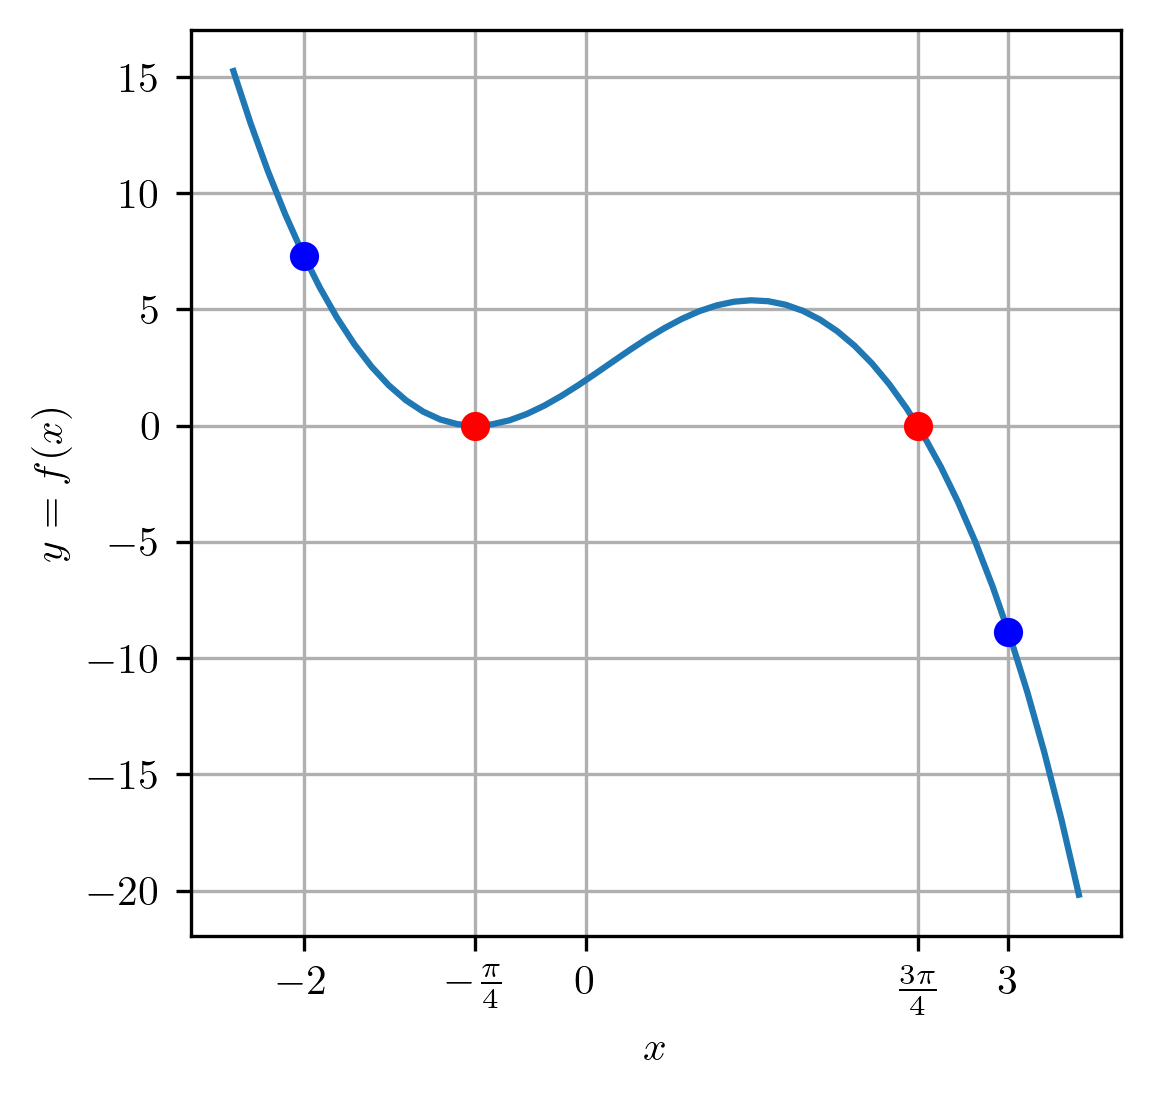
\includegraphics[width=0.8\textwidth]{./cap_eq1d/dados/fig_bis_intro/fig}
  \caption{Esboço da função $f$ do Exemplo~\ref{cap_eq1d_sec_bissec:ex:bis_intro}.}
  \label{cap_eq1d_sec_bissec:fig:bis_intro}
\end{figure}

Observamos que esta função é contínua e que, por exemplo, $f(-2)>0$ e $f(3)<0$, logo $f(-2)\cdot f(3) < 0$ e, de fato, $f$ tem pelo menos um zero\endnote{De fato, $f$ tem três zeros no intervalo $(-2, 3)$.} no intervalo $(-2, 3)$.
\end{ex}

Consideramos, então, uma função $f$ contínua tal que $f(a)\cdot f(b) < 0$. O \hl{Método da Bisseção é iterativo}, a primeira aproximação para uma solução de $f(x)=0$ é tomada como o ponto médio do intervalo $(a, b)$, i.e.
\begin{equation}
  x^{(0)} = \frac{a^{(1)}+b^{(1)}}{2},
\end{equation}
onde $a^{(0)} = a$ e $b^{(0)} = b$. Daí, se ocorrer $f(x^{(0)})=0$ o problema está resolvido. Caso contrário, $f$ tem pelo menos um zero num dos subintervalos $(a^{(0)}, x^{(0)})$ ou $(x^{(0)}, b^{(0)})$, pois $f(a^{(0)})\cdot f(x^{(0)}) < 0$ ou  $f(x^{(0)})\cdot f(b^{(0)}) < 0$, respectivamente e exclusivamente. No primeiro caso, escolhemos $(a^{(1)}, b^{(1)}) = (a^{(0)}, x^{(0)})$ ou, no segundo caso, tomamos $(a^{(1)}, b^{(1)}) = (x^{(0)}, b^{(0)})$. Então, a segunda aproximação para uma solução é computada como
\begin{equation}
  x^{(1)} = \frac{a^{(1)} + b^{(1)}}{2}.
\end{equation}
O procedimento se repete até obtermos uma aproximação com a precisão desejada.

\begin{ex}\label{cap_eq1d_sec_bissec:ex:bis_exec}
  Consideremos o problema de encontrar um zero da função
  \begin{equation}
    \begin{aligned}
      f(x) &= \sen^2\left(x+\frac{\pi}{4}\right) - x^3 \\
           &+ \frac{\pi}{4}x^2 + \frac{5\pi^2}{16}x + \frac{3\pi^3}{64}.
    \end{aligned}
\end{equation}
Do esboço de seu gráfico (Figura \ref{cap_eq1d_sec_bissec:fig:bis_intro}), observamos que $f(2)\cdot f(3) \neq 0$ sendo que o zero $x=3\pi/4\approx 2,3562$ de $f$ está no intervalo $(2, 3)$. Aplicando o Método da Bisseção com intervalo inicial $(a^{(0)}, b^{(0)}) = (2, 3)$ e aproximação inicial $x^{(0)} = (a^{(0)}+b^{(0)})/2$, obtemos as aproximações apresentadas na Tabela \ref{cap_eq1d_sec_bissec:tab:bis_exec}.

\begin{table}[h!]
  \centering
  \caption{Resultados referentes ao Exemplo~\ref{cap_eq1d_sec_bissec:ex:bis_exec}.}
  \begin{tabular}{r|rr|r|r}
    k & $a^{(k)}$ & $b^{(k)}$ & $x^{(k)}$ & $s$ \\\hline
    0 & $2,0000$ & $3,0000$ & $2,5000$ & -1 \\
    1 & $2,0000$ & $2,5000$ & $2,2500$ &  1 \\
    2 & $2,2500$ & $2,5000$ & $2,3750$ & -1 \\
    3 & $2,2500$ & $2,3750$ & $2,3125$ & 1 \\
    4 & $2,3125$ & $2,3750$ & $2,3438$ & 1 \\
    5 & $2,3438$ & $2,3750$ & $2,3594$ &  -1 \\
    6 & $2,3438$ & $2,3594$ & $2,3516$ & 1 \\
    7 & $2,3516$ & $2,3594$ & $2,3555$ &  1 \\
    8 & $2,3555$ & $2,3594$ & $2,3574$ &  -1 \\
    9 & $2,3555$ & $2,3574$ & $2,3564$ & -1 \\\hline
    \multicolumn{5}{r}{\small $s := f(a^{(k)})\cdot f(x^{(k)})$}
  \end{tabular}
  \label{cap_eq1d_sec_bissec:tab:bis_exec}
\end{table}

\begin{lstlisting}
import numpy as np

f = lambda x: np.sin(x+np.pi/4)**2 \
  - x**3 + np.pi/4*x**2 + 5*np.pi**2/16*x \
  + 3*np.pi**3/64

a = 2
b = 3
x = (a + b)/2
print(f"0: a={a:.4f}, b={b:.4f}, x={x:.4f}")
for k in range(9):
  s = np.sign(f(a)*f(x))
  if (s == -1):
    b = x
  elif (s == 1):
    a = x
  else:
    break
  x = (a + b)/2
  print(f"{k+1}: a={a:.4f}, b={b:.4f}, x={x:.4f}")
\end{lstlisting}

\end{ex}

\subsection{Análise Numérica}

Dada uma função contínua $f:[a, b]\to\mathbb{R}$ com $f(a)\cdot f(b) < 0$, vamos mostrar que o \hl{Método da Bisseção é \emph{globalmente convergente} e tem \emph{ordem de convergência linear}}.

\begin{defn}\normalfont{(\hl{Método Iterativo Globalmente Convergente}.)}
  Um método iterativo
  \begin{gather}
    x^{(0)} = \text{aprox. inicial},\\
    x^{(k+1)} = g\left(x^{k}\right),
  \end{gather}
  com $k = 0,1,\ldots$, é dito \emph{globalmente convergente}, quando
  \begin{equation}
    {\color{blue}\lim_{k\to\infty}\left|x^{(k+1)}-x^{(k)}\right| = 0}
  \end{equation}
  para qualquer escolha de $x^{(0)}$.
\end{defn}

\begin{defn}\normalfont{(\hl{Ordem de convergência}.)}
  Seja $\left(x^{(k)}\right)_{k=1}^\infty$ uma sequência convergente com
  \begin{equation}
    \lim_{k\to\infty} \left|x^{(k+1)}-x^{(k)}\right| = 0,
  \end{equation}
  com $x^{(k+1)}-x^{(k)}\neq 0$ para todo $k$. Dizemos que $\left(x^{(k)}\right)_{k=1}^\infty$ converge com ordem $\alpha>0$ e com constante de erro assintótica $C>0$, quando
  \begin{equation}
    {\color{blue}\lim_{k\to\infty}\frac{\left|x^{(k+1)}-x^*\right|}{\left|x^{(k)}-x^*\right|^\alpha} = C}. 
  \end{equation}
\end{defn}

Em geral, \hl{quando maior o valor de $\alpha$, mais rapidamente é a convergência das iteradas de um método iterativo}. Os seguintes casos são particularmente importantes:
\begin{itemize}
\item \hl{Se $\alpha = 1$ e $\lambda < 1$, o método é \emph{linearmente convergente}}.
\item \hl{Se $\alpha = 2$, o método é \emph{quadraticamente convergente}}.
\end{itemize}

\subsubsection{Convergência e Precisão}

\begin{teo}\label{cap_eq1d_sec_bissec:teo:convp}
  Seja $f:[a, b]\to\mathbb{R}$ função contínua com $f(a)\cdot f(b) < 0$. Então, o \hl{Método da Bisseção é globalmente convergente}.
\end{teo}
\begin{dem}
  Seja $(x^{(k)})_{k=1}^\infty$ a sequência de aproximações\endnote{Caso, $f\left(a^{(k)}\right)=0$ ou $f\left(a^{(b)}\right)=0$, então assumimos que $a^{(k+i)} = a^{(k)}$ ou $b^{(k+i)} = b^{(k)}$, conforme o caso, para $i=1,2,3,\ldots$.} do Método da Bisseção. Por construção, temos
  \begin{align}
    \left|x^{(k)} - x^{(k-1)}\right| &\leq b^{(k-1)}-a^{(k-1)}\\
                                     &\leq \frac{b^{(k-2)}-a^{(k-2)}}{2}\\
                                     &\vdots\\
                                     &\leq \frac{b^{(0)}-a^{(0)}}{2^{k-1}}
  \end{align}
  Ou seja, obtemos a \hl{\emph{estimativa de convergência}}
  \begin{equation}\label{cap_eq1d_sec_bissec:eq:estconvp}
    {\color{blue}\left|x^{(k)} - x^{(k-1)}\right| \leq \frac{b^{(0)}-a^{(0)}}{2^{k-1}}}
  \end{equation}
  Daí, segue que
  \begin{align}
    \lim_{k\to\infty} \left|x^{(k)}-x^{(k-1)}\right| &= \lim_{k\to\infty} b^{(k)}-a^{(k-1)}\\
                                                     &= 0.
  \end{align}
\end{dem}

\begin{ex}\label{cap_eq1d_sec_bissec:ex:bis_convp}
  No Exemplo \ref{cap_eq1d_sec_bissec:ex:bis_exec} aplicamos o Método da Bisseção para a função
  \begin{equation}
    \begin{aligned}
      f(x) &= \sen^2\left(x+\frac{\pi}{4}\right) - x^3 \\
           &+ \frac{\pi}{4}x^2 + \frac{5\pi^2}{16}x + \frac{3\pi^3}{64}.
    \end{aligned}
\end{equation}
no intervalo $(2, 3)$. Ao recuperarmos os valores de $\left|x^{(k)}-x^{(k-1)}\right|$ obtemos
\begin{center}
  \begin{tabular}[H]{l|l|r}
    $k$ & $x^{(k)}$ & $\left|x^{(k)}-x^{(k-1)}\right|$\\\hline
    $0$ & $2.5000$ & -x-\\
    $1$ & $2.2500$ & $2,5\times 10^{-1}$\\
    $2$ & $2,3750$ & $1,2\times 10^{-1}$\\
    $3$ & $2,3125$ & $6,2\times 10^{-2}$\\
    $4$ & $2,3438$ & $3,1\times 10^{-2}$\\
    $5$ & $2,3594$ & $1,6\times 10^{-2}$\\
    $6$ & $2,3516$ & $7,8\times 10^{-3}$\\
    $7$ & $2,3555$ & $3,9\times 10^{-3}$\\
    $8$ & $2,3574$ & $2,0\times 10^{-3}$\\
    $9$ & $2,3564$ & $9,8\times 10^{-4}$\\\hline
  \end{tabular}
\end{center}

Observamos que os valores estão de acordo com a estimativa de convergência \ref{cap_eq1d_sec_bissec:eq:estconvp}, donde
\begin{align}
  |x^{(9)}-x^{(8)}| &\leq \frac{b^{(0)}-a^{(0)}}{2^{9}}\\
                     &= \frac{3 - 2}{2^{9}} = 1.9\times 10^{-3}
\end{align}
\end{ex}

O \hl{Teorema~{\ref{cap_eq1d_sec_bissec:teo:convp}} nos garante a convergência do Método da Bisseção e uma estimativa de \emph{precisão}} (Equação~\ref{cap_eq1d_sec_bissec:eq:estconvp}). O teorema \hl{não garante que} o método \hl{converge para um zero da função objetivo}, apenas garante que as aproximações convergem para algum valor no intervalo inicial dado.

\subsubsection{Convergência e Exatidão}

Dada uma \hl{função contínua e estritamente monótona}\endnote{Função estritamente crescente ou estritamente decrescente, exclusivamente.} \hl{$f:[a, b]\to\mathbb{R}$ com $f(a)\cdot f(b) < 0$}, temos que o Método da Bisseção converge para o zero de $f$ em $[a, b]$.

\begin{teo}\label{cap_eq1d_sec_bissec:teo:bissece}
  Seja $f:[a, b]\to\mathbb{R}$ função contínua e estritamente monótona com $f(a)\cdot f(b) < 0$. Então, o \hl{Método da Bisseção converge para o zero de $f$ em $[a, b]$}.
\end{teo}
\begin{dem}
  Das hipóteses temos que $f$ tem um único zero $x^*$ em $(a, b)$. Seja $(x^{(k)})_{k=1}^\infty$ a sequência de aproximações\endnote{Caso, $f\left(a^{(k)}\right)=0$ ou $f\left(a^{(b)}\right)=0$, então assumimos que $a^{(k+i)} = a^{(k)}$ ou $b^{(k+i)} = b^{(k)}$, conforme o caso, para $i=1,2,3,\ldots$.} do Método da Bisseção. Por construção, temos
  \begin{align}
    |x^{(k)} - x^{*}| &\leq \frac{b^{(k)}-a^{(k)}}{2}\\
                      &\leq \frac{b^{(k-1)}-a^{(k-1)}}{2^2}\\
                      &\vdots \\
                      &\leq \frac{b^{(1)}-a^{(1)}}{2^k},
  \end{align}
  donde, obtemos a seguinte estimativa do \hl{\emph{erro de truncamento}}
  \begin{equation}\label{cap_eq1d_sec_bissec:eq:bis_est_trunc}
    {\color{blue}|x^{(k)} - x^{*}| \leq \frac{b^{(1)}-a^{(1)}}{2^k}}.
  \end{equation}
  E, daí também, segue que o método converge para o zero de $f$, pois
  \begin{equation}
    \lim_{k\to\infty} |x^{(k)}-x^{*}| = \lim_{k\to\infty} \frac{b^{(1)}-a^{(1)}}{2^k} = 0.
  \end{equation}
\end{dem}

\begin{obs}(\normalfont{\hl{Estimativa de Exatidão}.)}
  A estimativa de truncamento \ref{cap_eq1d_sec_bissec:eq:bis_est_trunc} é também um \emph{estimativa de exatidão}, i.e. nos fornece uma medida do erro na $k$-ésima aproximação do Método da Bisseção.
\end{obs}

\begin{ex}\label{cap_eq1d_sec_bissec:ex:bis_convp}
  No Exemplo \ref{cap_eq1d_sec_bissec:ex:bis_exec} aplicamos o Método da Bisseção para a função
  \begin{equation}
    \begin{aligned}
      f(x) &= \sen^2\left(x+\frac{\pi}{4}\right) - x^3 \\
           &+ \frac{\pi}{4}x^2 + \frac{5\pi^2}{16}x + \frac{3\pi^3}{64}.
    \end{aligned}
\end{equation}
no intervalo $(2, 3)$. A aplicação do método, nos fornece
\begin{center}
  \begin{tabular}[H]{llr}
    $k$ & $x^{(k)}$ & $\left|x^{(k)}-x^{*}\right|$\\\hline
    $0$ & $2.3560$ & $1.4\times 10^{-1}$ \\
    $1$ & $2.2500$ & $1.1\times 10^{-1}$ \\
    $2$ & $2.3750$ & $1.9\times 10^{-2}$ \\
    $3$ & $2.3125$ & $4.4\times 10^{-2}$ \\
    $4$ & $2.3438$ & $1.2\times 10^{-2}$ \\
    $5$ & $2.3594$ & $3.2\times 10^{-3}$ \\
    $6$ & $2.3516$ & $4.6\times 10^{-3}$ \\
    $7$ & $2.3555$ & $7.3\times 10^{-4}$ \\
    $8$ & $2.3574$ & $1.2\times 10^{-3}$ \\
    $9$ & $2.3564$ & $2.5\times 10^{-4}$ \\\hline
  \end{tabular}
\end{center}
onde, $x^* = x_1 = 3\pi/4$. Observamos que este resultado é consistente com a estimativa do erro de truncamento \eqref{cap_eq1d_sec_bissec:eq:bis_est_trunc}, da qual temos
\begin{align}
  |x^{(9)} - x^*| &\leq \frac{b^{(0)}-a^{(0)}}{2^{10}}\\
                  &= \frac{1}{2^{10}} = 1,0\E-3.
\end{align}
\end{ex}

\begin{obs}\normalfont{(\hl{Ordem de Convergência Linear}.)}
  A estimativa de convergência \eqref{cap_eq1d_sec_bissec:eq:bis_est_trunc} também pode ser usada para mostrarmos que, assintoticamente, o Método da Bisseção tem a seguinte taxa de convergência linear
  \begin{equation}
    \left|x^{(k+1)} - x^{(k)}\right| \lesssim \frac{1}{2}\left|x^{(k)} - x^{(k-1)}\right|^{\pmb{1}}.
  \end{equation}
\end{obs}

\subsection{Zeros de Multiplicidade Par}

Sejam \hl{$f$ uma função suave e $x^*$ um zero de multiplicidade par de $f$}. Observamos que o \hl{Método da Bisseção não é diretamente aplicável} para aproximar $x^*$. Isto ocorre, pois, neste caso, $x^*$ será um ponto de mínimo ou de máximo local de $f$, não havendo pontos $a$ e $b$ próximos de $x^*$ tal que $f(a)\cdot f(b) < 0$.

Agora, \hl{sendo $x^*$ um zero de $f$ de multiplicidade $2m$}, temos que ela admite a seguinte decomposição
\begin{equation}
  f(x) = (x-x^*)^{2m}g(x),
\end{equation}
onde $g$ é uma função suave e $g(x^*)\neq 0$. Daí, a derivada de $f$
\begin{equation}
  f'(x) = 2m(x-x^*)^{2m-1}g(x) + (x-x^*)^{2m}g'(x),
\end{equation}
tem $x^*$ como um zero de multiplicidade $2m-1$ (ímpar) e, desta forma, \hl{podemos aplicar o Método da Bisseção em $f'$ para aproximar $x^*$}.

\begin{ex}\label{cap_eq1d_sec_bissec:ex:bis_multpar}
  A função
  \begin{equation}
    \begin{aligned}
      f(x) &= \sen^2\left(x+\frac{\pi}{4}\right) - x^3 \\
           &+ \frac{\pi}{4}x^2 + \frac{5\pi^2}{16}x + \frac{3\pi^3}{64}.
    \end{aligned}
\end{equation}
tem $x=-\pi/4\approx -0,7854$ como um zero de multiplicidade par (veja Figura \ref{cap_eq1d_sec_bissec:fig:bis_multpar}).

\begin{figure}[H]
  \centering
  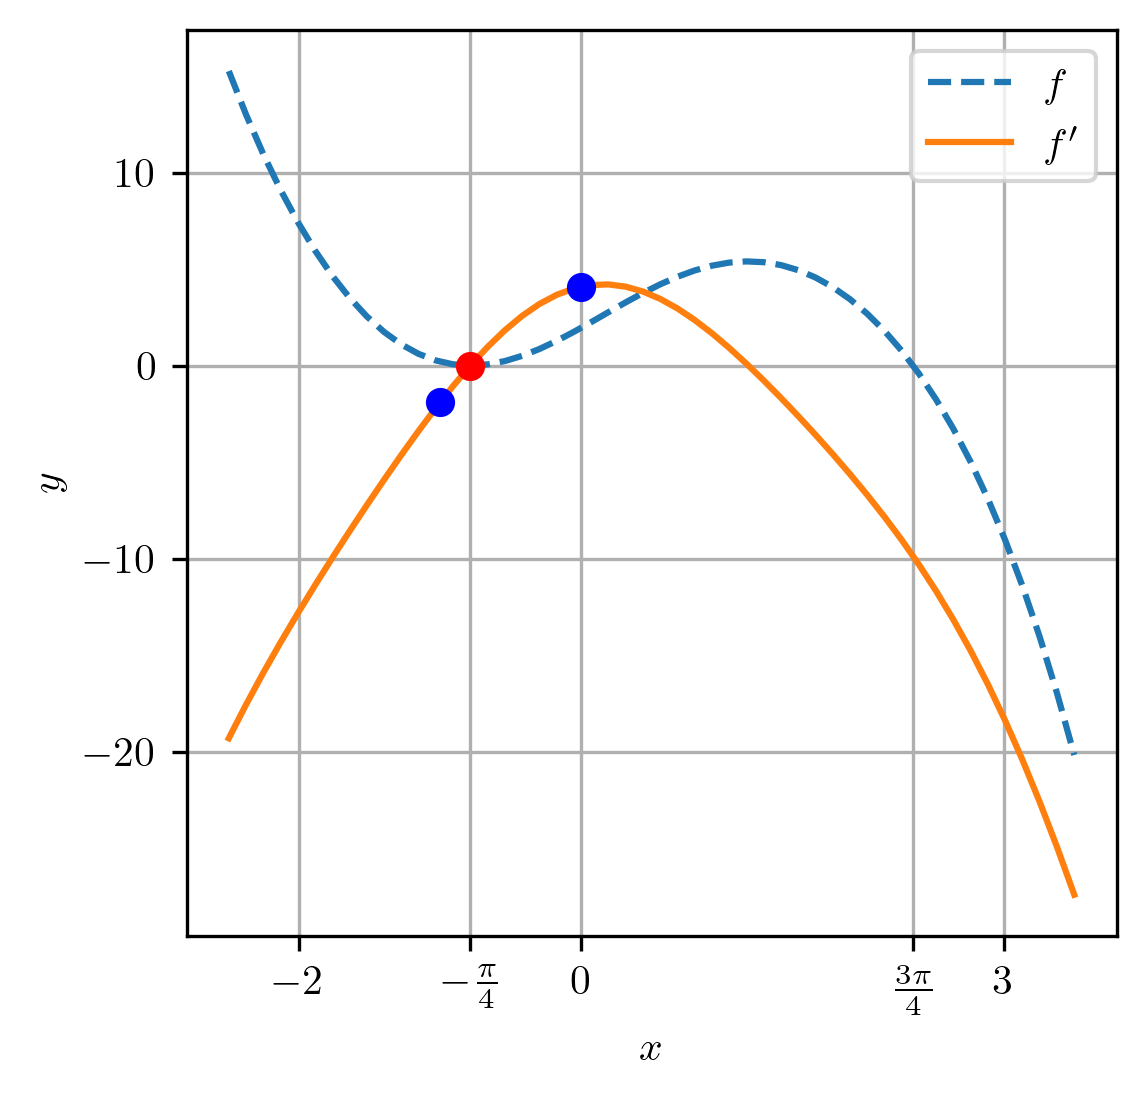
\includegraphics[width=0.8\textwidth]{./cap_eq1d/dados/fig_bis_multpar/fig}
  \caption{Esboço do gráfico da $f$ e de sua derivada $f'$ dada no Exemplo \ref{cap_eq1d_sec_bissec:ex:bis_multpar}.}
  \label{cap_eq1d_sec_bissec:fig:bis_multpar}
\end{figure}

Para aplicarmos o Método da Bisseção para aproximarmos este zero, primeiramente, derivamos $f$
\begin{equation}
  \begin{aligned}
    f'(x) &= 2\sin(x+\pi/4)\cos(x+\pi/4) - 3x^2 \\
          &+ \frac{\pi}{2}x + \frac{5\pi^2}{16}.
  \end{aligned}
\end{equation}
O esboço do gráfico de $f'$ (Figura \ref{cap_eq1d_sec_bissec:fig:bis_multpar}) mostra que $f'(-1)\cdot f'(0) < 0$ sendo que no intervalo $(-1, 0)$ $f'$ tem um zero de multiplicidade ímpar. Então, aplicando o Método da Bisseção a $f'$ no intervalo inicial $(a^{(1)}, b^{(1)}) = (-1, ~0)$, obtemos os resultados apresentados na Tabela~\ref{cap_eq1d_sec_bissec:tab:bis_multpar}. Nesta tabela são apresentados as iteradas até a convergência da solução com precisão de $10^{-3}$.

\begin{table}[H]
  \centering
  \caption{Resultados referentes ao Exemplo~\ref{cap_eq1d_sec_bissec:ex:bis_exec}.}
  \begin{tabular}{r|rr|r|r}
    k & $a^{(k)}$ & $b^{(k)}$ & $x^{(k)}$ & $s$\\\hline
    0 & $-1,0000\E+0$ & $0,0000\E+0$ & $-5,0000\E-1$ & -1 \\
    1 & $-1,0000\E+0$ & $-5,0000\E-1$ & $-7,5000\E-1$ & -1 \\
    2 & $-1,0000\E+0$ & $-7,5000\E-1$ & $-8,7500\E-1$ & 1 \\
    3 & $-8,7500\E-1$ & $-7,5000\E-1$ & $-8,1250\E-1$ &  1 \\
    4 & $-8,1250\E-1$ & $-7,5000\E-1$ & $-7,8125\E-1$ & -1 \\
    5 & $-8,1250\E-1$ & $-7,8125\E-1$ & $-7,9688\E-1$ & 1 \\
    6 & $-7,9688\E-1$ & $-7,8125\E-1$ & $-7,8906\E-1$ & 1 \\
    7 & $-7,8906\E-1$ & $-7,8125\E-1$ & $-7,8516\E-1$ & -1 \\
    8 & $-7,8906\E-1$ & $-7,8516\E-1$ & $-7,8711\E-1$ & 1 \\
    9 & $-7,8711\E-1$ & $-7,8516\E-1$ & $-7,8613\E-1$ & 1 \\\hline
    \multicolumn{5}{r}{\small $s := f'(a^{(k)})\cdot f'(x^{(k)})$}
  \end{tabular}
  \label{cap_eq1d_sec_bissec:tab:bis_multpar}
\end{table}
\end{ex}

\subsection{Exercícios}

\begin{exer}
  Use o Método da Bisseção para aproximar um zero de
  \begin{equation}
    f(x)=x^3\sen(x)-\cos(x)
\end{equation}
aplicando como intervalo inicial $(a^{(0)}, b^{(0)}) = (0,5, ~1)$ e aproximação inicial $x^{(0)}=(a^{(0)}+b^{(0)})/2$. Faça, então, $6$ iterações de forma a obter a aproximação $x^{(6)}$ e forneça-a com $7$ dígitos significativos por arredondamento.
\end{exer}
\begin{resp}
  $9,179688\times 10^{-1}$
\end{resp}

\begin{exer}
  Considere o Método da Bisseção para aproximar um zero de $f(x)=x^3\sen(x)-\cos(x)$, aplicando como intervalo inicial $(a^{(0)}, b^{(0)}) = (0,5, ~1)$ e aproximação inicial $x^{(0)}=(a^{(0)}+b^{(0)})/2$. Use a estimativa de convergência \eqref{cap_eq1d_sec_bissec:eq:bis_est_trunc}
  \begin{equation}
    \left|x^{(k)} - x^{*}\right| \leq \frac{b^{(1)}-a^{(1)}}{2^k},
  \end{equation}
para estimar o número mínimo de iterações $k_{conv}$ necessárias para se obter a solução com exatidão de $10^{-4}$. Então, compute $x^{(k_{conv})}$ e forneça-o com $6$ dígitos significativos por arredondamento.
\end{exer}
\begin{resp}
  $9,15833\E-1$
\end{resp}

\begin{exer}
  Use o Método da Bisseção para computar a(s) solução(ões) das seguintes equações com precisão de 8 dígitos significativos.
  \begin{enumerate}[a)]
  \item $x = 2^{-x}$ para $0\leq x \leq 2$.
  \item $e^{-x^2} = 3x - x^2$ para $-1\leq x\leq 4$.
  \end{enumerate}
\end{exer}
\begin{resp}
  a) $6.4118574\times 10^{-1}$; b) $3.3536470\times 10^{-1}$; $2.9999589$
\end{resp}

\begin{exer}
  Use o Método da Bisseção para encontrar uma aproximação com precisão de $10^{-4}$ do zero de
  \begin{align}
    f(x) &= (-x^2+1,154x-0,332929)\cos(x) + x^2 \nonumber\\
         &- 1,154x + 0,332929
  \end{align}
no intervalo $(0,55, ~0,65)$. Forneça a aproximação computada com $7$ dígitos significativos por arredondamento.
\end{exer}
\begin{resp}
  $5,770508\times 10^{-1}$
\end{resp}

\begin{exer}
  Aplique o Método da Bisseção para encontrar o ponto crítico\endnote{Definimos que $x$ é ponto crítico de uma dada $f$, quando $f'(x) = 0$ ou $\nexists f'(x)$.} de
  \begin{equation}
    f(x) = (1-x^2)e^{-x^2}
  \end{equation}
  no intervalo $(0, 2)$. Obtenha o resultado com precisão de $5$ dígitos significativos por arredondamento.
\end{exer}
\begin{resp}
  $1,4142\E+0$
\end{resp}

\ifisbook
\subsubsection{Respostas}
\shipoutAnswer
\fi

%%% SECTION %%%

\section{Método da Falsa Posição}\label{cap_eq1d_sec_falsapos}

O Método da Falsa Posição \hl{é uma variação do Método da Bisseção}. Dada uma função $f$ contínua, escolhemos um intervalo inicial $(a, b)$ tal que $f(a)\cdot f(b) < 0$ (i.e. \hl{$f$ tem sinais trocados nos pontos $a$ e $b$}). Então, uma \hl{aproximação para o zero de $f$} neste intervalo \hl{é computada como o ponto de interseção da reta secante a $f$ pelos pontos $(a, f(a))$ e $(b, f(b))$}, i.e.
\begin{equation}
  x = a - \frac{b-a}{f(b)-f(a)}f(a).
\end{equation}
Veja a Figura \ref{cap_eq1d_sec_falsapos:fig:falsapos}.

\begin{figure}[H]
  \centering
  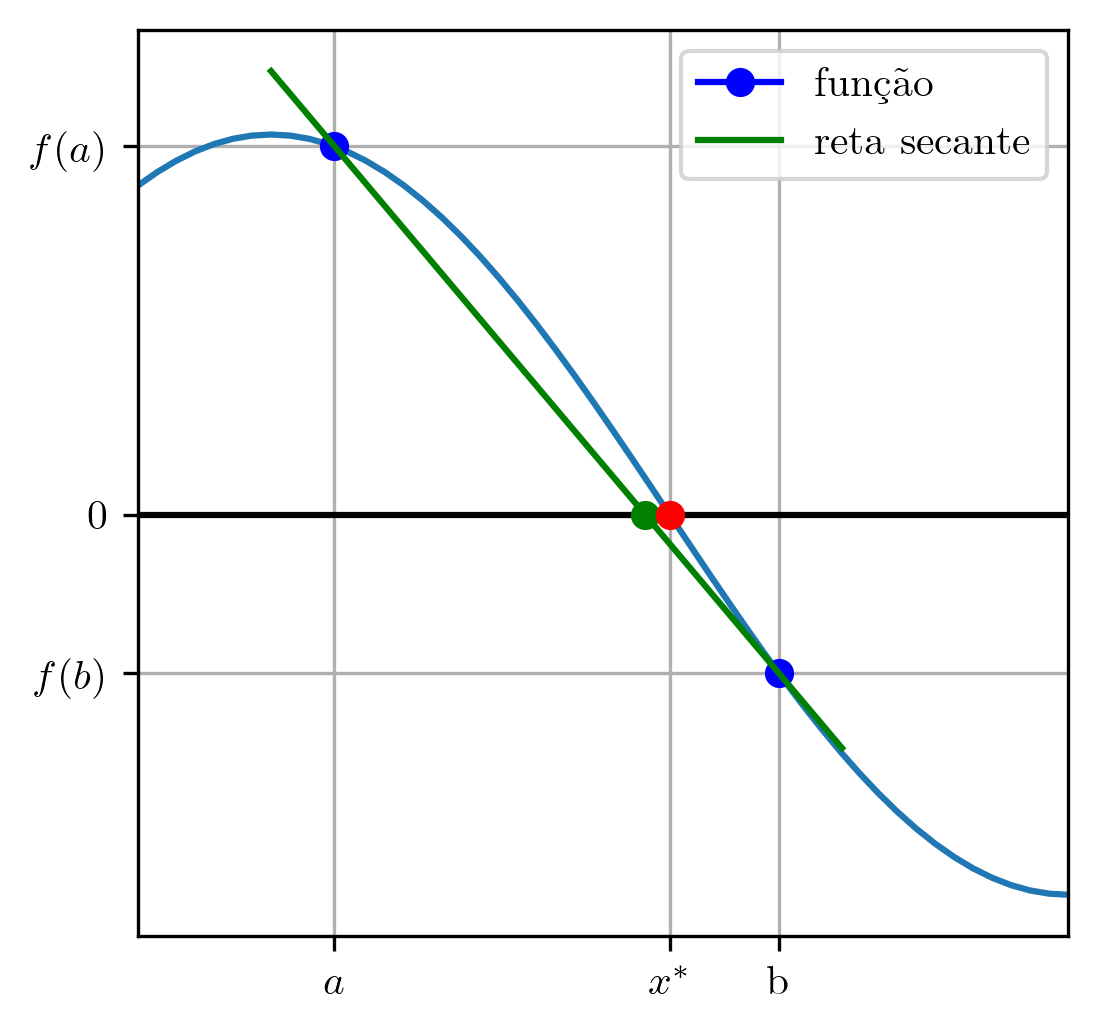
\includegraphics[width=0.7\textwidth]{./cap_eq1d/dados/fig_falsapos/fig}
  \caption{Ilustração do método da falsa posição.}
  \label{cap_eq1d_sec_falsapos:fig:falsapos}
\end{figure}

Mais explicitamente, \hl{o método consiste no seguinte procedimento iterativo}:
\begin{enumerate}
\item Determinar um intervalo $(a^{(1)}, b^{(1)})$ tal que $f(a^{(1)})\cdot f(b^{(1)}) < 0$.
\item Para $k = 1, 2, 3, \cdots, N$:
  \begin{enumerate}[2.1]
  \item $\displaystyle x^{(k)} = a^{(k)} - \frac{b^{(k)}-a^{(k)}}{f(b^{(k)})-f(a^{(k)})}f(a^{(k)})$
  \item Verificar critério de parada.
  \item Se $f(a^{(k)})\cdot f(x^{(k)}) < 0$, então $a^{(k+1)}=a^{(k)}$ e $b^{(k+1)}=x^{(k)}$.
  \item Se $f(x^{(k)})\cdot f(b^{(k)}) > 0$, então $a^{(k+1)}=x^{(k)}$ e $b^{(k+1)}=b^{(k)}$.
  \end{enumerate}
\end{enumerate}

\begin{ex}
  Consideremos o problema de aproximar o zero de
  \begin{equation}
    \begin{aligned}
      f(x) &= \sen^2\left(x+\frac{\pi}{4}\right) - x^3 \\
           &+ \frac{\pi}{4}x^2 + \frac{5\pi^2}{16}x + \frac{3\pi^3}{64}.
    \end{aligned}
\end{equation}
no intervalo $(0, 3)$. A tabela abaixo mostra os resultados obtidos da aplicação do Método da Falsa Posição com intervalo inicial $(a^{(1)}, b^{(1)}) = (2, 3)$. Aqui, o método foi iterado até a convergência com cinco dígitos significativos.

\begin{center}
  \begin{tabular}{r|rr|r|r}
    k & $a^{(k)}$ & $b^{(k)}$ & $x^{(k)}$ & $s$\\\hline
    1 & $2,0000$ & $3,0000$ & $2,2455$ & 1 \\
    2 & $2,2455$ & $3,0000$ & $2,3240$ &  1 \\
    3 & $2,3240$ & $3,0000$ & $2,3470$ & 1 \\
    4 & $2,3470$ & $3,0000$ & $2,3536$ & 1 \\
    5 & $2,3536$ & $3,0000$ & $2,3555$ & 1 \\
    6 & $2,3555$ & $3,0000$ & $2,3560$ & 1 \\
    7 & $2,3560$ & $3,0000$ & $2,3561$ &  1 \\
    8 & $2,3561$ & $3,0000$ & $2,3562$ & 1 \\
    9 & $2,3562$ & $3,0000$ & $2,3562$ & 1 \\
    10 & $2,3562$ & $3,0000$ & $2,3562$ & 1 \\\hline
    \multicolumn{5}{r}{\small $s := f'(a^{(k)})\cdot f'(x^{(k)})$}
  \end{tabular}
\end{center}

\begin{lstlisting}
import numpy as np

f = lambda x: np.sin(x+np.pi/4)**2 \
  - x**3 + np.pi/4*x**2 + 5*np.pi**2/16*x \
  + 3*np.pi**3/64

a = 2.
b = 3.
for k in range(10):
  x = a - (b-a)/(f(b)-f(a))*f(a)
  print(f"{k+1}: {x:.4f}")

  s = np.sign(f(a)*f(x))
  if (s == -1):
    b = x
  elif (s == 1):
    a = x
  else:
    break
\end{lstlisting}
\end{ex}

\begin{obs}\normalfont{(\hl{Ordem de Convergência}.)}
  O Método da Falsa Posição é \emph{globalmente convergente} e tem \emph{ordem de convergência linear} \cite[Seção 8.3]{Ralston2001a}.
\end{obs}

\subsection{Exercícios}

\begin{exer}
  Use o método da falsa posição para aproximar um zero de
  \begin{equation}
    f(x) = x^3\sen(x)-\cos(x)
  \end{equation}
  aplicando, como intervalo inicial $(a^{(1)}, b^{(1)}) = (0,5, ~1)$ e aproximação inicial
  \begin{equation}
    x^{(0} = a^{(1)} - \frac{b^{(1)}-a^{(1)}}{f(b^{(1)})-f(a^{(1)})}f(a^{(1)}).
  \end{equation}
  Faça, então, $4$ iterações deste método de forma a obter a aproximação $x^{(4)}$ e forneça-a com $7$ dígitos significativos por arredondamento.
\end{exer}
\begin{resp}
  $9,158079\times 10^{-1}$
\end{resp}

\begin{exer}
  Use o Método da Falsa Posição para computar a(s) solução(ões) das seguintes equações com precisão de 8 dígitos significativos.
  \begin{enumerate}[a)]
  \item $x = 2^{-x}$ para $0\leq x \leq 2$.
  \item $e^{-x^2} = 3x - x^2$ para $-1\leq x\leq 4$.
  \end{enumerate}
\end{exer}
\begin{resp}
  a) $6.4118574\times 10^{-1}$; b) $3.3536470\times 10^{-1}$; $2.9999589$
\end{resp}

\begin{exer}
  Use o Método da Falsa Posição para encontrar uma aproximação com precisão de $4$ dígitos significativos do zero de 
  \begin{equation}
    \begin{aligned}
      f(x) &= (-x^2+1,154x-0,332929)\cos(x) + x^2 \\
           &- 1,154x + 0,332929
    \end{aligned}
\end{equation}
  no intervalo $[-1, 0]$.
\end{exer}
\begin{resp}
  $-7,861\times 10^{-1}$
\end{resp}

\begin{exer}
  Use o Método da Falsa Posição para encontrar uma aproximação com precisão de $10^{-4}$ do zero de
  \begin{equation}
    \begin{aligned}
      f(x) &= (-x^2+1,154x-0,332929)\cos(x) + x^2 \\
           &- 1,154x + 0,332929
    \end{aligned}
\end{equation}
no intervalo $(0,55, ~0,65)$. Forneça a aproximação computada com $7$ dígitos significativos por arredondamento.
\end{exer}
\begin{resp}
  $5,770508\times 10^{-1}$
\end{resp}

\begin{exer}
  Aplique o Método da Falsa Posição para encontrar o ponto crítico\endnote{Definimos que $x$ é ponto crítico de uma dada $f$, quando $f'(x) = 0$ ou $\nexists f'(x)$.} de
  \begin{equation}
    f(x) = (1-x^2)e^{-x^2}
  \end{equation}
  no intervalo $(0, 2)$. Obtenha o resultado com precisão de $5$ dígitos significativos por arredondamento.
\end{exer}

\ifisbook
\subsubsection{Respostas}
\shipoutAnswer
\fi

%%% SECTION %%%

\section{Iteração de Ponto Fixo}\label{cap_eq1d_sec_pfixo}

\hl{Um \emph{ponto fixo de uma função} $g$ é um ponto $x$ tal que}
\begin{equation}\hleq
  g(x) = x.
\end{equation}
Geometricamente, \hl{pontos fixos são interseções do gráfico da $g$ com a reta $y=x$}, veja a Figura \ref{cap_eq1d_sec_pfixo:fig:pfixo}.

\begin{figure}[H]
  \centering
  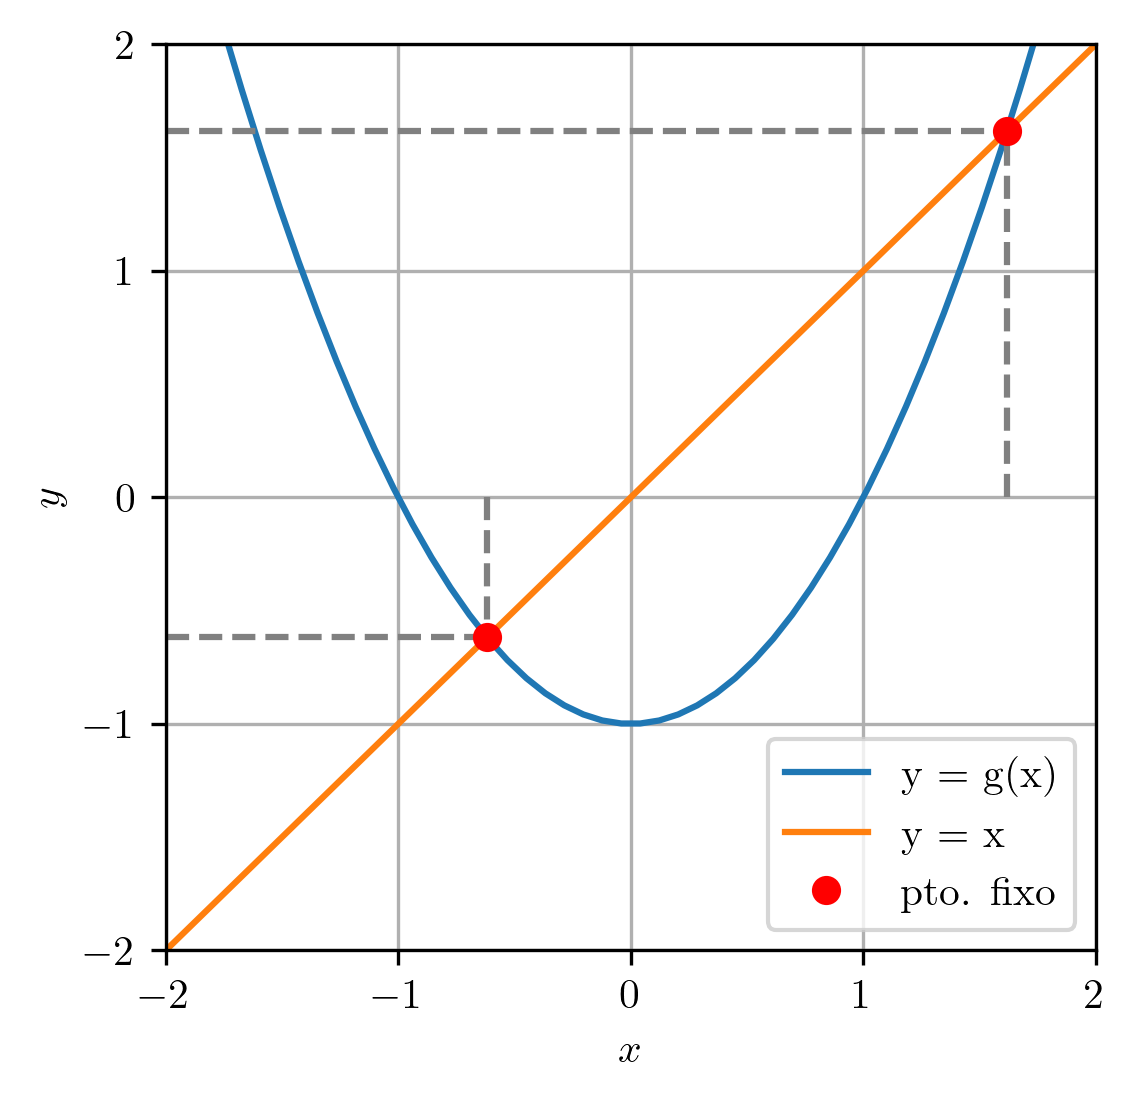
\includegraphics[width=0.8\textwidth]{./cap_eq1d/dados/fig_pfixo/fig}
  \caption{Exemplos de pontos fixos.}
  \label{cap_eq1d_sec_pfixo:fig:pfixo}
\end{figure}

Observamos que \hl{toda equação de uma incógnita pode ser reescrita} de forma equivalente \hl{como um problema de ponto fixo}.

\begin{ex}\label{cap_eq1d_sec_pfixo:ex:pfixo_intro}
  Consideremos o problema de resolver
  \begin{equation}
    \begin{aligned}
      &\sen^2\left(x+\frac{\pi}{4}\right) = x^3 - \frac{\pi}{4}x^2 \\
      &\qquad - \frac{5\pi^2}{16}x - \frac{3\pi^3}{64}.
    \end{aligned}
\end{equation}
Podemos reescrevê-la como o problema de se obter os zeros da seguinte função
\begin{equation}
  \begin{aligned}
    f(x) &= \sen^2\left(x+\frac{\pi}{4}\right) - x^3 \\
         &+ \frac{\pi}{4}x^2 + \frac{5\pi^2}{16}x + \frac{3\pi^3}{64}.
  \end{aligned}
\end{equation}
Por sua vez, este problema é equivalente aos seguintes problemas de ponto fixo (entre outros):
\begin{enumerate}[a)]
\item
  \begin{equation}
    \begin{aligned}
      g_1(x) &= \frac{16}{5\pi^2}\left[-\sen^2\left(x+\frac{\pi}{4}\right) + x^3 \right. \\
             &\left. - \frac{\pi}{4}x^2 - \frac{3\pi^3}{64}\right] = x.
    \end{aligned}
  \end{equation}
\item
  \begin{equation}
    \begin{aligned}
      g_2(x) &= \left[\sen^2\left(x+\frac{\pi}{4}\right) + \frac{\pi}{4}x^2\right. \\
             &\left. + \frac{5\pi^2}{16}x + \frac{3\pi^3}{64}\right]^{\frac{1}{3}} = x
    \end{aligned}
\end{equation}
\end{enumerate}
Na Figura \ref{cap_eq1d_sec_pfixo:fig:ex_pfixo_intro} podemos observar que os zeros da $f$ (a saber, $x_1=3\pi/4\approx 2,3562$ e $x_2=x_3=-\pi/4\approx -0,78540$) coincidem com os pontos fixos das funções $g_1$ e $g_2$.

\begin{figure}[H]
  \centering
  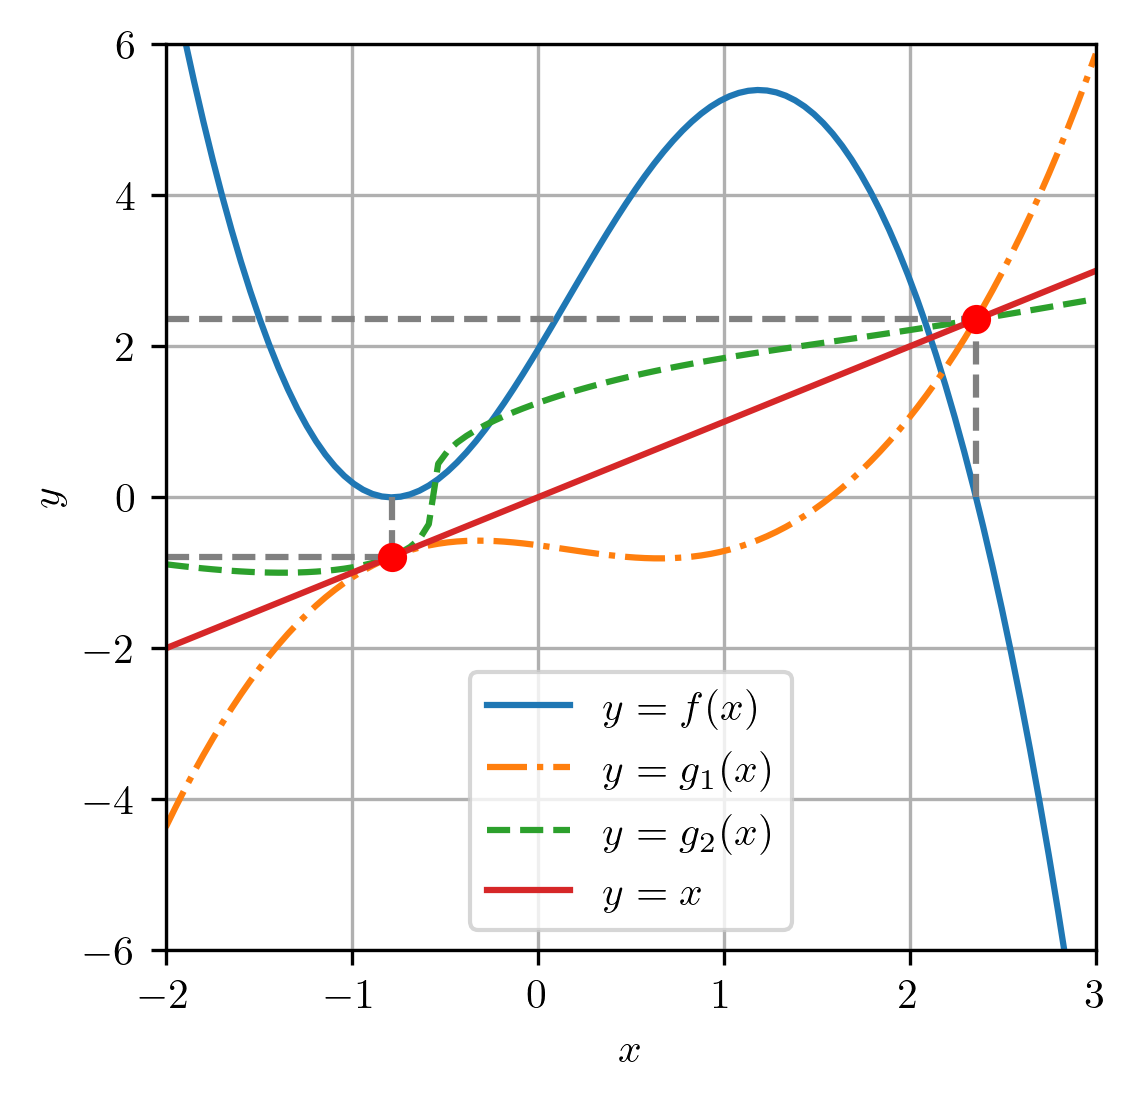
\includegraphics[width=0.8\textwidth]{./cap_eq1d/dados/fig_ex_pfixo_intro/fig}
  \caption{Esboço da função $f$, $g_1$ e $g_2$ do Exemplo~\ref{cap_eq1d_sec_pfixo:ex:pfixo_intro}.}
  \label{cap_eq1d_sec_pfixo:fig:ex_pfixo_intro}
\end{figure}
\end{ex}

Em muitos casos, é possível obter aproximações de um ponto fixo de uma dada função $g$ pela chamada \hl{\emph{iteração de ponto fixo}}:
\begin{align}
  {\color{blue}x^{(0)}} &{\color{blue}= \text{aprox. inicial}},\\
  {\color{blue}x^{(k+1)}} &{\color{blue}= g(x^{(k)})},
\end{align}
com $k=0,1,2,\ldots$.

\begin{ex}
  Vamos estudar as seguintes iterações de ponto fixo com as funções $g1$ e $g_2$ consideradas no Exemplo~\ref{cap_eq1d_sec_pfixo:ex:pfixo_intro}.
  \begin{enumerate}[a)]
  \item Função $g_1$ com $x^{(0)} = 0,7$.
    \begin{align}
      x^{(0)} &= -0,70000,\\
      x^{(1)} &= g_1\left(x^{(0)}\right)\\
              &= -0,70959,\\
      x^{(2)} &= g_1\left(x^{(1)}\right)\\
              &=-0,71716,\\
              &\vdots \nonumber\\
      x^{(99)} &= g_1\left(x^{(98)}\right)\\
              &= -0,77862,\\
              &\vdots \nonumber\\
      x^{(999)} &= g_1\left(x^{(998)}\right)\\
              &= -0,78466,\\    
              &\vdots \nonumber\\
      x^{(19999)} &= g_1\left(x^{(19998)}\right)\\
              &= -0,78536.
    \end{align}
    Neste caso as iterações de ponto fixo convergem (lentamente) para o ponto fixo $x=-\pi/4\approx -0,78540$.

  \item Função $g1$ com $x^{(0)} = 2,5$.
    
    Este valor inicial está próximo do ponto fixo $x=3\pi/4\approx 2,3562$, entretanto as iterações de ponto fixo divergem:
    \begin{align}
      x^{(0)} &= 2,50000,\\
      x^{(1)} &= g_1\left(x^{(0)}\right)\\
              &= 2,9966,\\
      x^{(2)} &= 5,8509,\\
              &\vdots \nonumber\\
      x^{(7)} &= 4,8921\times 10^{121}.
    \end{align}
    
  \item Função $g_2$ com $x^{(0)} = 2,5$.
    Neste caso, as iterações de ponto fixo convergem (rapidamente) para o ponto fixo próximo:
    \begin{align}
      x^{(0)} &= 2,50000,\\
      x^{(1)} &= g_2\left(x^{(0)}\right)\\
              &= 2,4155,\\
      x^{(2)} &= 2,3805,\\
              &\vdots \\
      x^{(9)} &= 2,3562.
    \end{align}    
  \end{enumerate}
\end{ex}

Este último exemplo mostra que a iteração do ponto fixo nem sempre é convergente. Antes de vermos condições suficientes para a convergência, vejamos sua interpretação geométrica.

\subsection{Interpretação Geométrica}

A Figura \ref{cap_eq1d_sec_pfixo:fig:pfixo_interp} apresenta o caso de uma iteração de ponto fixo convergente. As iterações iniciam-se no ponto $x^{(0)}$ e seguem para $x^{(1)} = g(x^{(0)})$ e $x^{(2)} = g(x^{(1)})$.

\begin{figure}[H]
  \centering
  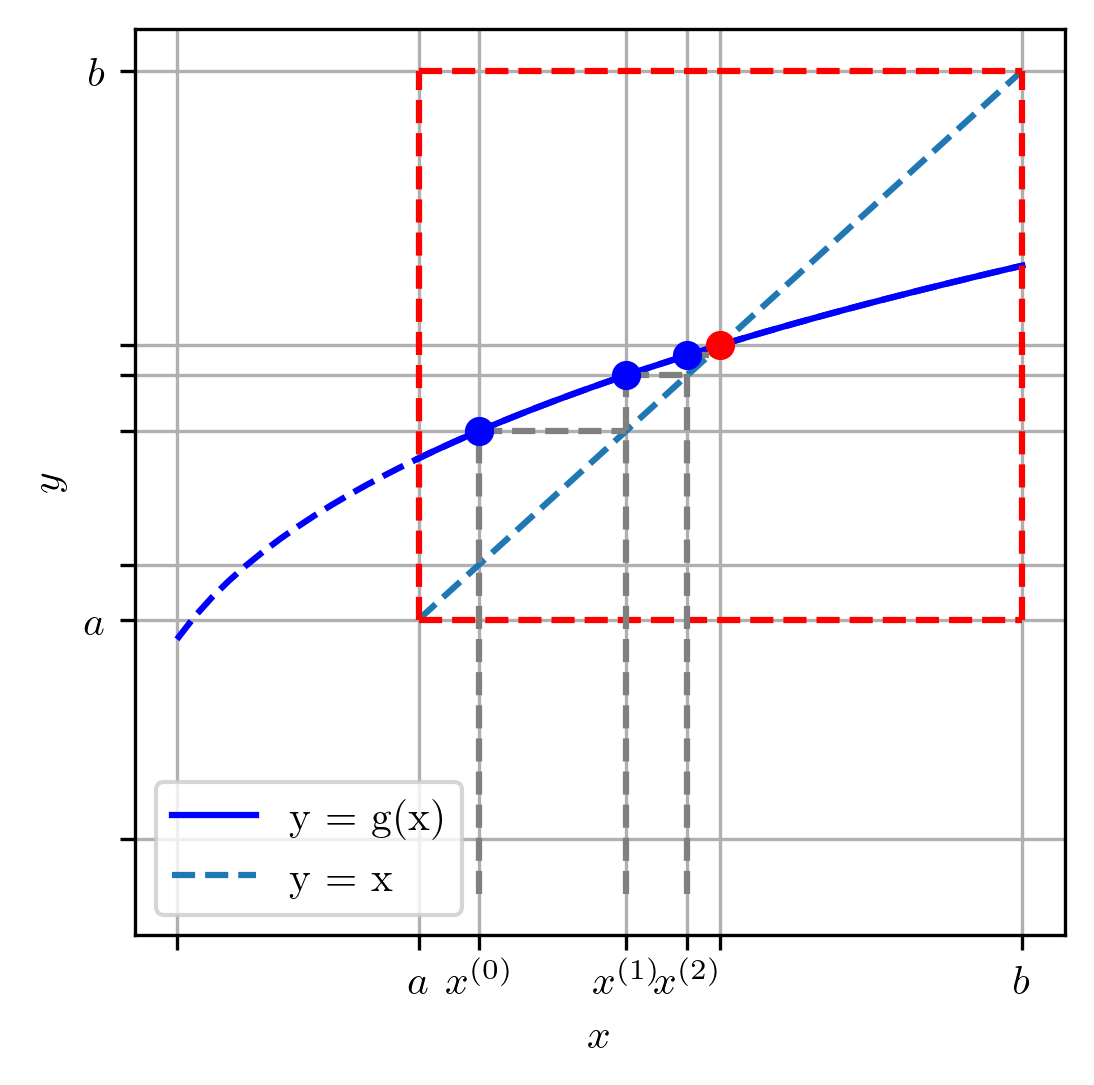
\includegraphics[width=\textwidth]{./cap_eq1d/dados/fig_pfixo_interp/fig}
  \caption{Interpretação geométrica da iteração de ponto fixo.}
  \label{cap_eq1d_sec_pfixo:fig:pfixo_interp}
\end{figure}

\subsection{Análise Numérica}

O seguinte teorema nos fornece condições suficientes para a convergência das iterações de ponto fixo.

\begin{teo}\normalfont{(\hl{Teorema do Ponto Fixo}.)}\label{cap_eq1d_sec_pfixo:teo:pfixo}
  Seja $g$ função continuamente diferenciável satisfazendo ambas as seguintes condições
  \begin{enumerate}[a)]
  \item $g\left([a, b]\right) \subset [a, b]$,
  \item $|g'(x)|<K<1$ para todo $x\in [a, b]$.
  \end{enumerate}
  Então, $g$ tem um único ponto fixo $x^*\in [a, b]$ e as iterações
  \begin{equation}
    x^{(k+1)}= g\left(x^{(k)}\right), k=0, 1, 2, \ldots,
  \end{equation}
  convergem para $x^*$, para qualquer escolha de $x^{(0)}\in [a, b]$.
\end{teo}
\begin{dem}
  Da hipótese b), temos que $g$ é uma contração com
  \begin{equation}
    \left|g(x) - g(y)\right| < K\cdot |x - y|,
  \end{equation}
  para quaisquer $x,y\in [a, b]$. Com isso, da hipótese a) e tomando $x^{(0)}\in [a, b]$, temos
  \begin{align}
    \left|x^{(k+1)} - x^{(k)}\right| &= \left|g(x^{(k)}) - g(x^{(k-1)})\right|\\
                                     &\leq K \left|x^{(k)} - x^{(k-1)}\right|\\
                                     &\vdots \nonumber\\
                                     &\leq K^{k-1}\left|x^{(2)}-x^{(1)}\right|,
  \end{align}
  para $k=1, 2, \ldots$. Como $K<1$, temos $\left|x^{(k+1)}-x^{(k)}\right|\to 0$ quando $k\to\infty$ e, portanto, $x^{(k)}$ converge para algum $x^*\in [a, b]$.
  
  De fato, $x^*$ é ponto fixo de $g$, pois da continuidade da $g$, temos
  \begin{align}
    x^* &= \lim_{k\to\infty} x^{(k+1)}\\
        &= \lim_{k\to\infty} g(x^{(k)}) = g(x^*).
  \end{align}
  
  Por fim, $x^*$ é único, pois assumindo a existência de outro ponto fixo $x^{**}\neq x^*$ teríamos
  \begin{align}
    |x^* - x^{**}| &= |g(x^*) - g(x^{**})| \\
                   &< K|x^* - x^{**}|\\
                   &< |x^* - x^{**}|.
  \end{align}
\end{dem}

\begin{obs}\normalfont{(Ordem de Convergência.)}
  A \hl{iteração de ponto fixo tem ordem de convergência linear}
  \begin{equation}
    |x^{(k+1)} - x^{(k)}| < K|x^{(k)} - x^{(k-1)}|^{\pmb{1}},
  \end{equation}
onde $0 < K < 1$ é a constante dada na hipótese $b)$ do Teorema do Ponto Fixo. Além disso, isso mostra que \hl{quanto menor o valor da constante $K$, mais rápida é a convergência} das iterações de ponto fixo.
\end{obs}


\subsection{Zero de Funções}

Dado um problema de encontrar um zero de uma função $f$ (i.e., \hl{resolver $f(x)=0$}), podemos \hl{construir uma função $g$ com ponto fixo no zero de $f$} e aplicarmos a iteração de ponto fixo para computá-lo. Para tanto, observamos que
\begin{gather}
  {\color{blue}f(x) = 0} \\
  \Leftrightarrow \\
  \underbrace{{\color{blue}x - \alpha f(x)}}_{\color{blue}=: g(x)} = x,
\end{gather}
com $\alpha\in\mathbb{R}$ escolhido de forma a satisfazer as hipóteses do Teorema do Ponto Fixo (Teorema \ref{cap_eq1d_sec_pfixo:teo:pfixo}).

\begin{ex}\label{cap_eq1d_sec_pfixo:ex:pfixo_exec}
  Retornamos ao problema de encontrar o zero da função
  \begin{equation}
    f(x) = \sen^2\left(x+\frac{\pi}{4}\right) - x^3 + \frac{\pi}{4}x^2 + \frac{5\pi^2}{16}x + \frac{3\pi^3}{64}.
  \end{equation}
  no intervalo $[2,3]$. Para construir uma função $g$ para a iteração de ponto fixo neste intervalo, podemos tomar
  \begin{equation}
    g(x) = x - \alpha f(x),
  \end{equation}
com $\alpha = -0,1$. A Figura \ref{cap_eq1d_sec_pfixo:fig:ex_pfixo_exec} mostra esboços dos gráficos de $g$ e $|g'|$ no intervalos $[2, 3]$ e podemos observar que esta escolha de $\alpha$ faz com que a $g$ satisfaça o Teorema do Ponto Fixo.

\begin{figure}[H]
  \centering
  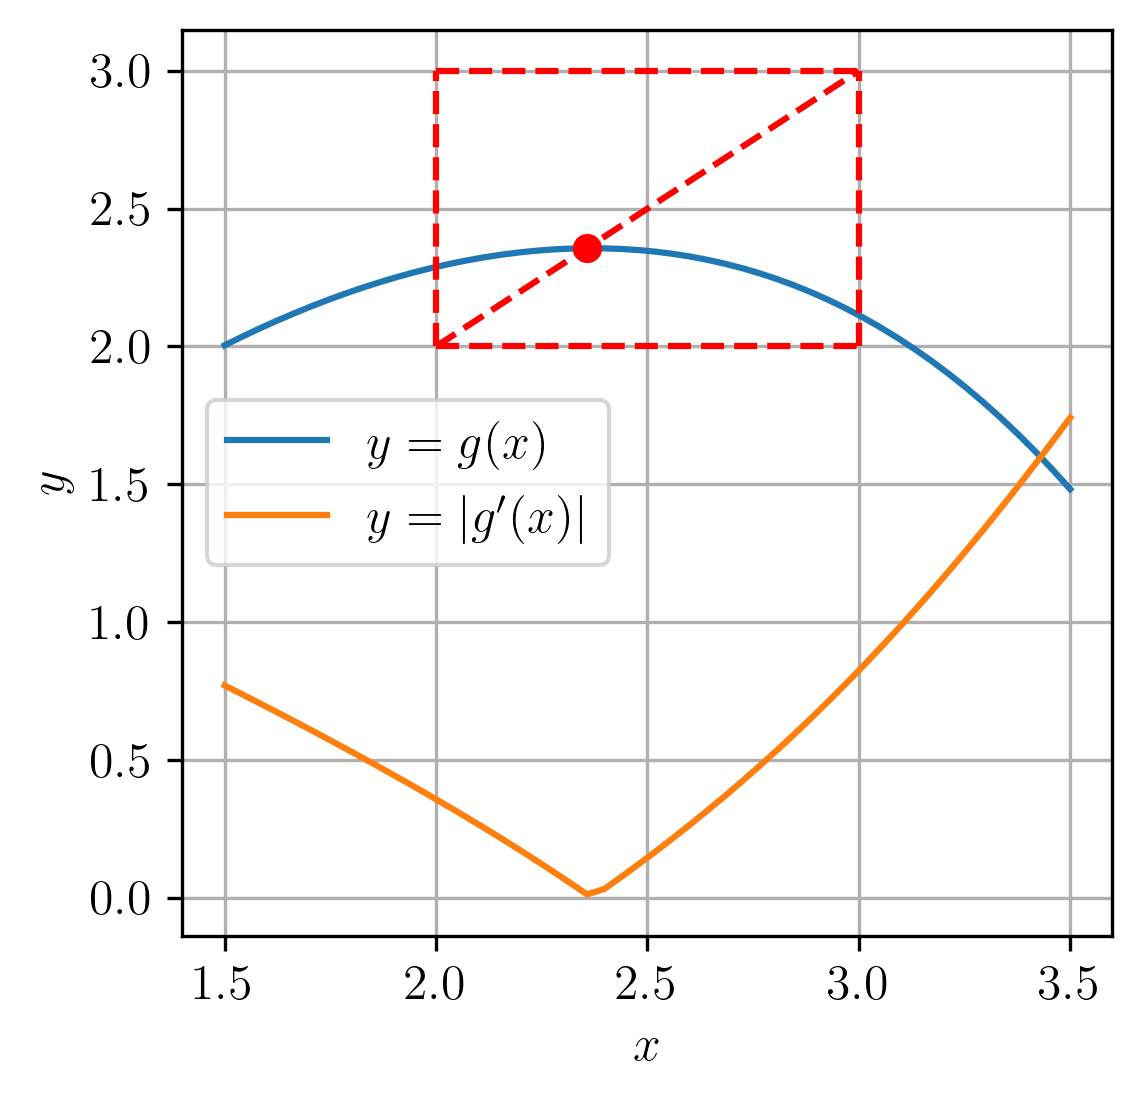
\includegraphics[width=\textwidth]{./cap_eq1d/dados/fig_ex_pfixo_exec/fig}
  \caption{Esboço dos gráficos de $g$ e $|g'|$ discutidas no Exemplo \ref{cap_eq1d_sec_pfixo:ex:pfixo_exec}.}
  \label{cap_eq1d_sec_pfixo:fig:ex_pfixo_exec}
\end{figure}

Então, fazendo as iterações de ponto fixo com aproximação inicial $x^{(0)}=2,6$, obtemos os resultados apresentados na Tabela \ref{cap_eq1d_sec_pfixo:tab:ex_pfixo_exec}.

\begin{table}[H]
  \centering
  \caption{Resultados referentes ao Exemplo \ref{cap_eq1d_sec_pfixo:ex:pfixo_exec}.}
  \label{cap_eq1d_sec_pfixo:tab:ex_pfixo_exec}
  \begin{tabular}{r|cc}
    $k$ & $x^{(k)}$ & $|x^{(k)}-x^{(k-1)}|$ \\\hline
    0 & $2,6000$ & -x-\\
    1 & $2,3264$ & $2,7\E-1$ \\
    2 & $2,3553$ & $2,9\E-2$ \\
    3 & $2,3562$ & $8,4\E-4$ \\
    4 & $2,3562$ & $1,1\E-5$ \\\hline
  \end{tabular}
\end{table}

\begin{lstlisting}
import numpy as np

# fun obj
f = lambda x: np.sin(x+np.pi/4)**2 \
  - x**3 + np.pi/4*x**2 + 5*np.pi**2/16*x \
  + 3*np.pi**3/64

# param
alpha = -0.1
# fun pto fixo
g = lambda x: x - alpha*f(x)

# aprox inicial
x0 = 2.6
print(f'\n{1}: {x0:.4f}')
for k in range(4):
  x = g(x0)
  nd = np.fabs(x-x0)
  print(f'{k+1}: {x:.4f}, {nd:.1e}')
  x0 = x
\end{lstlisting}

\end{ex}

\subsection{Exercícios}

\begin{exer}
  Forneça o(s) ponto(s) fixo(s) de
  \begin{equation}
    g(x) = x^2e^{-x^2}.
  \end{equation}
\end{exer}
\begin{resp}
  $x=0$
\end{resp}

\begin{exer}
  Verifique se a iteração de ponto fixo é convergente para as seguintes funções e aproximações iniciais:
  \begin{enumerate}[a)]
  \item $g_1(x) = \cos(x)$, $x^{(1)} = 0,5$
  \item $g_2(x) = x^2$, $x^{(1)} = 1,01$
  \end{enumerate}
  Justifique sua resposta.
\end{exer}
\begin{resp}
  a) Convergente; b) Divergente.
\end{resp}

\begin{exer}
  Considere o problema de computar uma aproximação do zero de $f(x)=x-\cos(x)$. Resolva-o aplicando a iteração de ponto fixo para a função auxiliar
  \begin{equation}
    g(x) = x - \alpha f(x),
  \end{equation}
restrita ao intervalo $[a, b] = [0.5, 1]$ com aproximação inicial $x^{(0)}=(a+b)/2$. Escolha o melhor valor de $\alpha$ entre os seguintes:
\begin{enumerate}
\item $\alpha = 1$
\item $\alpha = 0,5$
\item $\alpha = -0,5$
\item $\alpha = 0,6$
\end{enumerate}
Então, compute uma aproximação do zero de $f$ com $5$ dígitos significativos de precisão.
\end{exer}
\begin{resp}
  $\alpha=0,6$; $7,3909\times 10^{-1}$
\end{resp}

\begin{exer}
  Seja
  \begin{equation}
    \begin{aligned}
      f(x) &= \sen^2\left(x+\frac{\pi}{4}\right) - x^3\\
      &+ \frac{\pi}{4}x^2 + \frac{5\pi^2}{16}x + \frac{3\pi^3}{64}.
    \end{aligned}
\end{equation}
  \begin{enumerate}[a)]
  \item Aplique a iteração de ponto fixo na função auxiliar
    \begin{equation}
      g(x) = x - \alpha f(x)
    \end{equation}
    para algum $\alpha$ adequado, de forma que aproximação inicial $x^{(0)}=-0,5$ leve a iterações de ponto fixo que convirjam para $x^*=-\pi/4$, zero de multiplicidade par de $f$.
  \item Mostre que $g'(x^*) = 1$ para qualquer valor de $\alpha$. Por que isso explica a lenta convergência observada no item a)?
  \item Alternativamente, verifique que a abordagem da iteração de ponto fixo converge muito mais rápido para $x^*$ se aplicada à derivada de $f$, i.e. aplicando a iteração à função auxiliar
    \begin{equation}
      h(x) = x - \alpha f'(x),
    \end{equation}
    para um valor de $\alpha$ adequado.
  \end{enumerate}
\end{exer}
\begin{resp}
  a) $\alpha = 0.25$; b) Pois, não há $\alpha$ que satisfaz o Teorema do Ponto Fixo.; c) $\alpha = 0.1$
\end{resp}

\begin{exer}
  Use o Método da Iteração de Ponto Fixo para aproximar um zero de
  \begin{equation}
    f(x)=x^3\sen(x)-\cos(x)
  \end{equation}
  no intervalo inicial $[0,5, 1]$.
\end{exer}

\begin{exer}
  Use o Método da Iteração de Ponto Fixo para computar a(s) solução(ões) das seguintes equações com precisão de 8 dígitos significativos.
  \begin{enumerate}[a)]
  \item $x = 2^{-x}$ para $0\leq x \leq 2$.
  \item $e^{-x^2} = 3x - x^2$ para $-1\leq x\leq 4$.
  \end{enumerate}
\end{exer}
\begin{resp}
  a) $6.4118574\times 10^{-1}$; b) $3.3536470\times 10^{-1}$; $2.9999589$
\end{resp}

\begin{exer}
  Use o Método de Iteração de Ponto Fixo para encontrar uma aproximação com precisão de $4$ dígitos significativos do zero de 
  \begin{equation}
    \begin{aligned}
      f(x) &= (-x^2+1,154x-0,332929)\cos(x) + x^2 \\
      &- 1,154x + 0,332929
  \end{aligned}
  \end{equation}
  no intervalo $[-1, 0]$.
\end{exer}
\begin{resp}
  $-7,861\times 10^{-1}$
\end{resp}

\begin{exer}
  Use o Método de Iteração de Ponto Fixo para encontrar uma aproximação com precisão de $10^{-4}$ do zero de
  \begin{equation}
    \begin{aligned}
      f(x) &= (-x^2+1,154x-0,332929)\cos(x) + x^2\\
      &- 1,154x + 0,332929
  \end{aligned}
  \end{equation}
no intervalo $(0,55, ~0,65)$. Forneça a aproximação computada com $7$ dígitos significativos por arredondamento.
\end{exer}
\begin{resp}
  $5,770508\times 10^{-1}$
\end{resp}

\begin{exer}
  Use o Método da Iteração de Ponto Fixo para encontrar o ponto crítico\endnote{Definimos que $x$ é ponto crítico de uma dada $f$, quando $f'(x) = 0$ ou $\nexists f'(x)$.} de
  \begin{equation}
    f(x) = (1-x^2)e^{-x^2}
  \end{equation}
  no intervalo $(0, 2)$. Obtenha o resultado com precisão de $5$ dígitos significativos por arredondamento.
\end{exer}

\ifisbook
\subsubsection{Respostas}
\shipoutAnswer
\fi

%%% SECTION %%%

\section{Método de Steffensen}\label{cap_eq1d_sec_Steffensen}

O método de Steffensen\endnote{Johan Frederik Steffensen, 1873 - 1961, matemático e estatístico dinamarquês. Fonte: \href{https://pt.wikipedia.org/wiki/Johan_Frederik_Steffensen}{Wikipédia}.} é uma \hl{aplicação do método de aceleração de convergência $\Delta^2$ de Aitken}\endnote{Alexander Aitken, 1895 - 1967, matemático neozelandês. Fonte: \href{https://pt.wikipedia.org/wiki/Alexander_Aitken}{Wikipédia}.} \hl{à iteração de ponto fixo}.

\subsection{Acelerador $\Delta^2$ de Aitken}

Seja dada uma sequência $(x^{(k)})_{k=1}^\infty$ monotonicamente convergente para $x^*$. Assumimos que $k$ seja suficientemente grande tal que
\begin{equation}
  \frac{x^{(k+1)}-x^*}{x^{(k)}-x^*} \approx \frac{x^{(k+2)}-x^*}{x^{(k+1)}-x^*}.
\end{equation}
Então, isolando $x^*$ obtemos
\begin{equation}
  x^* \approx \frac{x^{(k)}x^{(k+2)}-(x^{(k+1)})^2}{x^{(k)}-2x^{(k+1)}+x^{(k+2)}}.
\end{equation}
Ainda, somando e subtraindo $(x^{(k)})^2$ e $2x^{(k)}x^{(k+1)}$ no numerador acima e rearranjando os termos, obtemos
\begin{equation}
  x^* \approx x^{(k)} - \frac{(x^{(k+1)}-x^{(k)})^2}{x^{(k+2)}-2x^{(k+1)}+x^{(k)}}.
\end{equation}

O observado acima, nos motiva a introduzir o \hl{acelerador $\Delta^2$ de Aitken}
\begin{equation}\label{cap_eq1d_sec_Steffensen:eq:ac_aitken}
  {\color{blue}\Delta^2\{x^{(k)},x^{(k+1)},x^{(k+2)}\} := x^{(k)} - \frac{(x^{(k+1)}-x^{(k)})^2}{x^{(k+2)}-2x^{(k+1)}+x^{(k)}}}.
\end{equation}


\begin{ex}\label{cap_eq1d_sec_Steffensen:ex:Aitken}
  Consideremos o problema de encontrar o zero da função
  \begin{equation}
    \begin{aligned}
      f(x) &= \sen^2\left(x+\frac{\pi}{4}\right) - x^3 \\
      &+ \frac{\pi}{4}x^2 + \frac{5\pi^2}{16}x + \frac{3\pi^3}{64}.
  \end{aligned}
  \end{equation}
  no intervalo $[2,3]$. Para tanto, podemos aplicar a iteração de ponto fixo dada por
  \begin{equation}
    \begin{aligned}
      x^{(k+1)} &= g(x^{(k)}) \\
      &:= x^{(k)} - \alpha f(x^{(k)}),\quad k=1,2,\ldots,
  \end{aligned}
  \end{equation}
com $\alpha=-0,05$ e $x^{(0)}=2,6$. Na Tabela \ref{cap_eq1d_sec_Steffensen:tab:ex_Aitken} temos os valores das iteradas $x^{(k)}$ e das correções $\Delta^2 = \Delta^2\{x^{(k)},x^{(k+1)},x^{(k+2)}\}$ de Aitken. Neste caso, a aceleração de convergência é notável.

\begin{table}[H]
  \centering
  \caption{Resultados referentes ao Exemplo \ref{cap_eq1d_sec_Steffensen:ex:Aitken}.}
  \label{cap_eq1d_sec_Steffensen:tab:ex_Aitken}
  \begin{tabular}{r|cc}
    $k$ & $x^{(k)}$ & $\Delta^2$ \\\hline
    0 & $2,6000$ & -x- \\
    1 & $2,4632$ & -x- \\
    2 & $2,4073$ & $2,3687$ \\
    3 & $2,3814$ & $2,3590$ \\
    4 & $2,3688$ & $2,3569$ \\
    5 & $2,3625$ & $2,3564$ \\
    6 & $2,3594$ & $2,3562$ \\
    7 & $2,3578$ & $2,3562$ \\\hline
  \end{tabular}
\end{table}

\begin{lstlisting}
import numpy as np

# fun obj
f = lambda x: np.sin(x+np.pi/4)**2 \
  - x**3 + np.pi/4*x**2 + 5*np.pi**2/16*x \
  + 3*np.pi**3/64

# fun pto fixo
alpha = -0.05
g = lambda x: x - alpha*f(x)

x0 = 2.6
print(f'\n1: {x0:.4f}')
for k in range(7):
  x1 = g(x0)
  x2 = g(x1)
  x = x0 - (x1-x0)**2/(x2-2*x1+x0)
  print(f'\n{k+2}: {x1:.4f}, {x:.4f}')
  x0 = x1
\end{lstlisting}

\end{ex}

\subsection{Análise Numérica}

\begin{defn}\normalfont{(Diferença Progressiva.)}
  Para uma sequência $\left(x^{(k)}\right)_{k=1}^\infty$, $\Delta x^{(k)}$ denota o \hl{\emph{operador de diferença progressiva}} e é definido por
  \begin{equation}
    \Delta x^{(k)} := x^{(k+1)} - x^{(k)}
  \end{equation}
  Potências maiores do operador são definidas recursivamente por
  \begin{equation}
    \Delta^n x^{(k)} = \Delta\left(\Delta^{n-1}x^{(k)}\right),\quad n\geq 2.
  \end{equation}
\end{defn}

Da definição acima, temos que
\begin{align}
  \Delta^2 x^{(k)} &:= \Delta\left(\delta x^{(k)}\right)\\
                   &= \Delta\left(x^{(k+1)} - x^{(k)}\right)\\
                   &= \Delta x^{(k+1)} - \Delta x^{(k)}\\
                   &= \left(x^{(k+2)} - x^{(k+1)}\right) - \left(x^{(k+1)} - x^{(k)}\right)\\
                   &= x^{(k+2)} - 2x^{(k+1)} + x^{(k)}
\end{align}
Com isso, temos que o \hl{acelerador $\Delta^2$ de Aitken} \eqref{cap_eq1d_sec_Steffensen:eq:ac_aitken} pode ser reescrito como
\begin{equation}
  {\color{blue}\Delta^2\left\{x^{(k)}, x^{(k+1)}, x^{(k+2)}\right\} := x^{(k)} - \frac{\left(\Delta x^{(k)}\right)^2}{\Delta^2 x^{(k)}}}.
\end{equation}

\begin{teo}
  \hl{Seja $\left(x^{(k)}\right)_{k=1}^\infty$ uma sequência linearmente convergente} para $x^*$ e
  \begin{equation}\label{cap_eq1d_sec_Steffensen:eq:teo_aux}
    \lim_{k\to\infty}\frac{x^{(k+1)}-x^*}{x^{(k)}-x^*} < 1.
  \end{equation}
  Então, \hl{a sequência $\Delta^2$ de Aitken} $\left(\hat{x}^{(k)}\right)_{k=1}^\infty$, com
  \begin{equation}
    \hat{x}^{(k)} := \Delta^2\left\{x^{(k)}, x^{(k+1)}, x^{(k+2)}\right\},
  \end{equation}
  \hl{converge} para $x^*$ \hl{mais rápido que $\left(x^{(k)}\right)$} no sentido de que
  \begin{equation}
    \lim_{k\to\infty}\frac{\hat{x}^{(k)}-x^*}{x^{(k)}-x^*} = 0.
  \end{equation}
\end{teo}
\begin{dem}
  \emconstrucao
\end{dem}

\subsection{Algoritmo de Steffensen}

O método de Steffensen \hl{consiste em aplicar o acelerador $\Delta^2$ de Aitken à iteração de ponto fixo}. Mais especificamente, sejam uma aproximação inicial $x^{(0)}$ e uma iteração de ponto fixo
\begin{equation}
  x^{(k+1)} = g(x^{(k)}),\quad k=0, 1, 2, \ldots.
\end{equation}
O algoritmo de Steffensen consiste em:
\begin{enumerate}
\item $x \leftarrow x^{(0)}$.
\item Para $k=0, 1, 2, \dotsc, N-1$:
  \begin{enumerate}
  \item $x_1 \leftarrow g(x)$.
  \item $x_2 \leftarrow g(x_1)$.
  \item $x^{(k+1)} \leftarrow \Delta^2\{x,x_1,x_2\}$.
  \item $x \leftarrow x^{(k+1)}$.
  \end{enumerate}
\end{enumerate}


\begin{ex}\label{cap_eq1d_sec_Steffensen:ex:Steffensen_exec}
  Retornamos ao exemplo anterior (Exemplo \ref{cap_eq1d_sec_Steffensen:ex:Aitken}. Na Tabela \ref{cap_eq1d_sec_Steffensen:tab:ex_Steffensen_exec} temos os valores das iteradas de Steffensen $x^{(k)}$ e do indicador de convergência $|x^{(k)}-x^{(k-1)}|$.

\begin{table}[h!]
  \centering
  \caption{Resultados referentes ao Exemplo \ref{cap_eq1d_sec_Steffensen:ex:Steffensen_exec}.}
  \label{cap_eq1d_sec_Steffensen:tab:ex_Steffensen_exec}
  \begin{tabular}{r|cc}
    $k$ & $x^{(k)}$ & $|x^{(k)}-x^{(k-1)}|$ \\\hline
    0 & $2,6000$ & -x- \\
    1 & $2,3687$ & $2,3\E-1$ \\
    2 & $2.3562$ & $1,2\E-2$ \\
    3 & $2,3562$ & $4,2\E-5$ \\\hline
  \end{tabular}
\end{table}

\begin{lstlisting}
import numpy as np

# fun obj
f = lambda x: np.sin(x+np.pi/4)**2 \
  - x**3 + np.pi/4*x**2 + 5*np.pi**2/16*x \
  + 3*np.pi**3/64

# fun pto fixo
alpha = -0.05
g = lambda x: x - alpha*f(x)

x0 = 2.6
print(f'\n1: {x0:.4f}')
for k in range(3):
  x1 = g(x0)
  x2 = g(x1)
  x = x0 - (x1-x0)**2/(x2-2*x1+x0)
  nd = np.fabs(x-x0)
  print(f'\n{k+2}: {x:.4f}, {nd:.1e}')
  x0 = x
\end{lstlisting}

\end{ex}

\subsection*{Exercícios}

\begin{exer}
  Use o método de Steffensen para obter uma aproximação do zero de $f(x)=x^3\sen(x)-\cos(x)$ no intervalo $[0,5, 1]$ com precisão de $10^{-6}$.
\end{exer}
\begin{resp}
    $9,15811\times 10^{-1}$
\end{resp}

\begin{exer}
  Use o Método da Iteração de Ponto Fixo para aproximar um zero de
  \begin{equation}
    f(x)=x^3\sen(x)-\cos(x)
  \end{equation}
  no intervalo inicial $[0,5, 1]$.
\end{exer}

\begin{exer}
  Use o Método de Steffensen para computar a(s) solução(ões) das seguintes equações com precisão de 8 dígitos significativos.
  \begin{enumerate}[a)]
  \item $x = 2^{-x}$ para $0\leq x \leq 2$.
  \item $e^{-x^2} = 3x - x^2$ para $-1\leq x\leq 4$.
  \end{enumerate}
\end{exer}
\begin{resp}
  a) $6.4118574\times 10^{-1}$; b) $3.3536470\times 10^{-1}$; $2.9999589$
\end{resp}

\begin{exer}
  Use o Método de Steffensen para encontrar uma aproximação com precisão de $4$ dígitos significativos do zero de 
  \begin{equation}
    f(x) = (-x^2+1,154x-0,332929)\cos(x) + x^2 - 1,154x + 0,332929
  \end{equation}
  no intervalo $[-1, 0]$.
\end{exer}
\begin{resp}
  $-7,861\times 10^{-1}$
\end{resp}

\begin{exer}
  Use o Método de Steffensen para encontrar uma aproximação com precisão de $10^{-4}$ do zero de
  \begin{equation}
    \begin{aligned}
      f(x) &= (-x^2+1,154x-0,332929)\cos(x) + x^2 \\
      &- 1,154x + 0,332929
  \end{aligned}
  \end{equation}
no intervalo $(0,55, ~0,65)$. Forneça a aproximação computada com $7$ dígitos significativos por arredondamento.
\end{exer}
\begin{resp}
  $5,770508\times 10^{-1}$
\end{resp}

\begin{exer}
  Use o Método de Steffensen para encontrar o ponto crítico\endnote{Definimos que $x$ é ponto crítico de uma dada $f$, quando $f'(x) = 0$ ou $\nexists f'(x)$.} de
  \begin{equation}
    f(x) = (1-x^2)e^{-x^2}
  \end{equation}
  no intervalo $(0, 2)$. Obtenha o resultado com precisão de $5$ dígitos significativos por arredondamento.
\end{exer}

\ifisbook
\subsubsection{Respostas}
\shipoutAnswer
\fi

%%% SECTION %%%

\section{Método de Newton}\label{cap_eq1d_sec_newton}

Seja $x^*$ um zero de uma dada função $f$, i.e.
\begin{equation}
  f(x^*)=0.
\end{equation}
A expansão em polinômio de Taylor{\taylor} de $f$ em um ponto $\tilde{x}$ dado, é
\begin{equation}
  f(x^*) = f(\tilde{x}) + f'(\tilde{x})(x^*-\tilde{x}) + O(|x^*-\tilde{x}|^2).
\end{equation}
Como $f(x^*)=0$, temos
\begin{gather}
  0 = f(\tilde{x}) + f'(\tilde{x})(x^*-\tilde{x}) + O((x^*-\tilde{x})^2)\\
  x^* + O(|x^*-\tilde{x}|^2) = \tilde{x} - \frac{f(\tilde{x})}{f'(\tilde{x})}
\end{gather}
Esta última expressão nos indica que \hl{dada uma aproximação $\tilde{x}$ do zero de $f$ a expressão}
\begin{equation}
  \hleq{\tilde{x} - \frac{f(\tilde{x})}{f'(\tilde{x})}},
\end{equation}
\hl{aproxima $x^*$ com um erro da ordem de $|x^*-\tilde{x}|^2$}.

Estas observações nos levam a \hl{\emph{iteração de Newton}}\endnote{Sir Isaac Newton, matemático e físico inglês, 1642 - 1726/27. Fonte: \href{https://en.wikipedia.org/wiki/Isaac_Newton}{Wikipedia}.}\index{iteração de!Newton}
\begin{align}
  \hleq{x^{(0)}} &\hleq{= \text{aprox. inicial}},\\
  \hleq{x^{(k+1)}} &\hleq{= x^{(k)} - \frac{f(x^{(k)})}{f'(x^{(k)})}},\label{cap_eq1d_sec_newton:eq:Newton_iteracao}
\end{align}
com $k=0, 1, 2, \ldots$.

\begin{ex}\label{cap_eq1d_sec_newton:ex:newton}
  Consideramos o problema de encontrar o zero da função
  \begin{equation}
    \begin{aligned}
      f(x) &= \sen^2\left(x+\frac{\pi}{4}\right) - x^3 \\
      &+ \frac{\pi}{4}x^2 + \frac{5\pi^2}{16}x + \frac{3\pi^3}{64}.
    \end{aligned}
  \end{equation}
  no intervalo $[2,3]$ (Consulte a Figura~\ref{cap_eq1d_sec_newton:fig:newton_ex}).

  \begin{figure}[H]
    \centering
    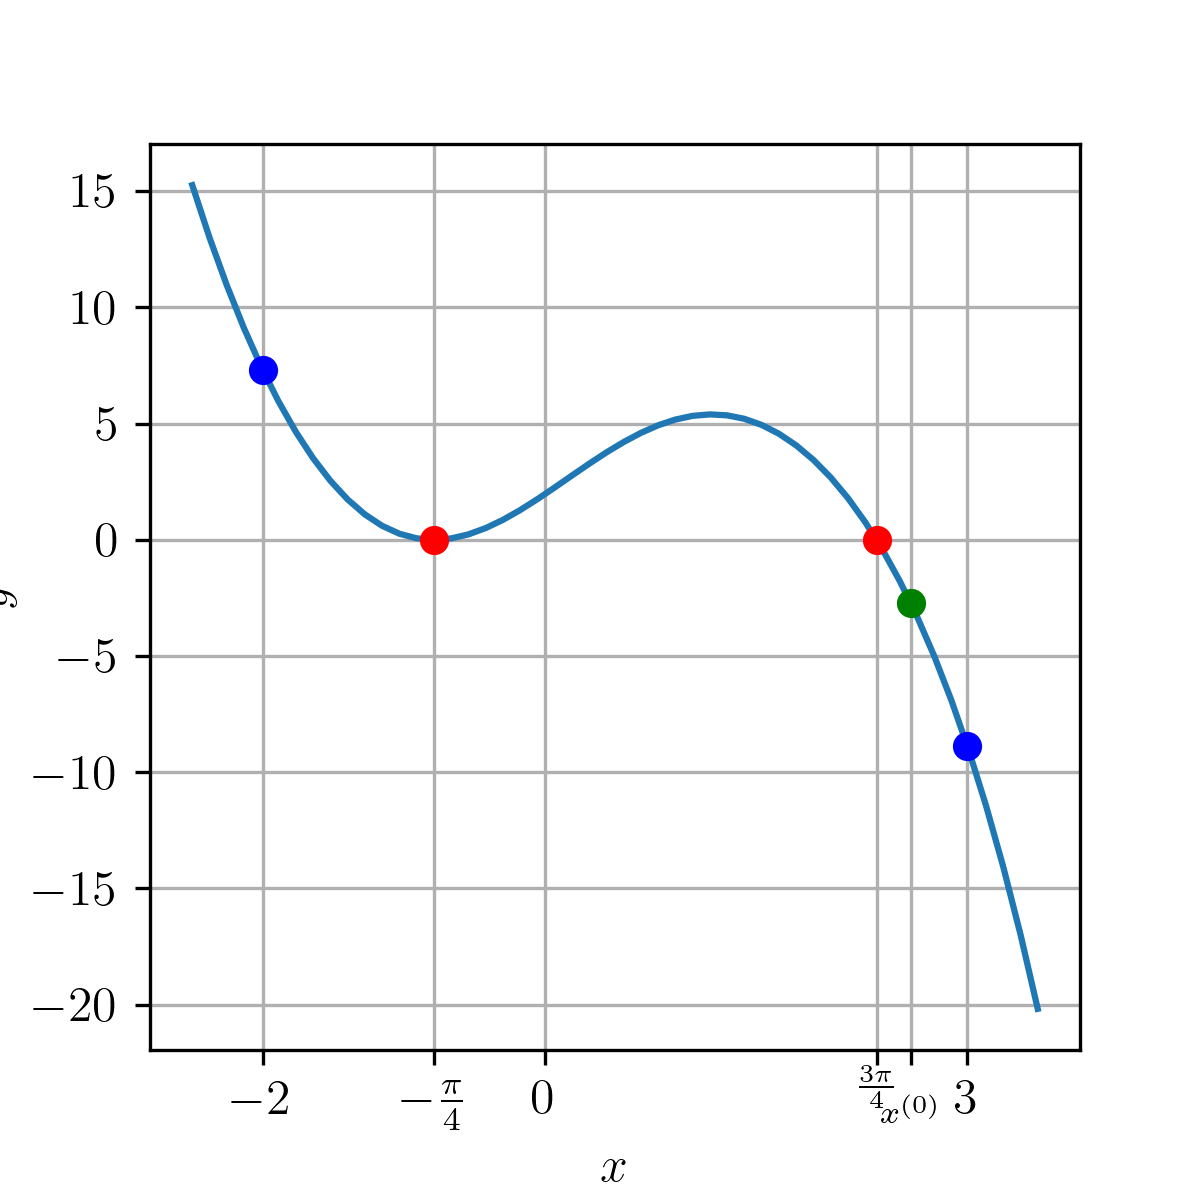
\includegraphics[width=0.8\textwidth]{./cap_eq1d/dados/fig_newton_ex/fig}
    \caption{Esboço da função $f$ do Exemplo~\ref{cap_eq1d_sec_newton:ex:newton}.}
  \label{cap_eq1d_sec_newton:fig:newton_ex}
\end{figure}


  Fazendo as iterações de Newton com aproximação inicial $x^{(0)}=2,6$, obtemos os resultados apresentados na Tabela \ref{tab:ex_Newton_exec}.

  \begin{table}[h!]
    \centering
    \caption{Resultados referentes ao Exemplo~\ref{cap_eq1d_sec_newton:ex:newton}.}
    \label{tab:ex_Newton_exec}
    \begin{tabular}{r|cc}
      $k$ & $x^{(k)}$ & $|x^{(k)}-x^{(k-1)}|$ \\\hline
      0 & $2,6000$ & -x-\\
      1 & $2,3836$ & $2,2\E-1$ \\
      2 & $2,3566$ & $2,7\E-2$ \\
      3 & $2,3562$ & $3,9\E-4$ \\
      4 & $2,3562$ & $8,3\E-8$ \\\hline
    \end{tabular}
  \end{table}

\begin{lstlisting}
import numpy as np

# fun obj
f = lambda x: np.sin(x+np.pi/4)**2 \
  - x**3 + np.pi/4*x**2 + 5*np.pi**2/16*x \
  + 3*np.pi**3/64

fl = lambda x: 2*np.sin(x+np.pi/4)*np.cos(x+np.pi/4) \
  -3*x**2 + np.pi/2*x + 5*np.pi**2/16

# aprox. inicial
x0 = 2.6
print(f'0: {x0:.4e}')

# iterações
for k in range(4):
  x = x0 - f(x0)/fl(x0)
  print(f'{k+1}: {x:.4e}')
  x0 = x
\end{lstlisting}

\end{ex}

\begin{obs}
  \hl{O método de Newton é uma iteração de ponto fixo ótima}. Do Teorema do Ponto Fixo (Teorema~\ref{cap_eq1d_sec_pfixo:teo:pfixo}), a iteração
  \begin{align}
    x^{k+1} &= g(x^{(k)})\\
            &:= x^{(k)} -\alpha f(x)\label{cap_eq1d_sec_pfixo:eq:Newton_pfixo}
  \end{align}
tem taxa de convergência\endnote{Supondo verdadeiras as demais hipóteses do Teorema~\ref{cap_eq1d_sec_pfixo:teo:pfixo}.}
\begin{equation}
  |x^{(k+1)}-x^{(k)}| \leq K |x^{(k)}-x^{(k-1)}|,
\end{equation}
com $K$ tal que $|g'(x)| = |1 - \alpha f'(x)| < K < 1$. Isto nos indica que a melhor escolha para $\alpha$ é
\begin{equation}
  \alpha = \frac{1}{f'(x)},
\end{equation}
de forma que \eqref{cap_eq1d_sec_pfixo:eq:Newton_pfixo} coincide com a iteração de \eqref{cap_eq1d_sec_newton:eq:Newton_iteracao}.
\end{obs}

\subsection{Interpretação Geométrica}

Dadas uma aproximação $x^{(k)}$ de um zero de uma função $f$, a iteração de Newton fornece uma nova aproximação $x^{(k+1)}$ com
\begin{equation}
  x^{(k+1)} = x^{(k)} - \frac{f(x^{(k)})}{f'(x^{(k)})}.
\end{equation}
Subtraindo $x^{(k+1)}$ e multiplicando por $-f'(x^{(k)})$, obtemos
\begin{equation}\label{cap_eq1d_sec_newton:eq:Newton_geointerp}
  0 = f'(x^{(k)})(x^{(k+1)}-x^{(k)}) + f(x^{(k)}),
\end{equation}
Observemos que o lado direito desta última equação corresponde a expressão da reta tangente ao gráfico de $f$ pelo ponto $(x^{(k)}, f(x^{(k)}))$, avaliada em $x^{(k+1)}$. Mais precisamente, a equação desta reta tangente é
\begin{equation}
  y = f'(x^{(k)})(x-x^{(k)}) + f(x^{(k)})
\end{equation}
e a equação \eqref{cap_eq1d_sec_newton:eq:Newton_geointerp} nos informa que em $x=x^{(k+1)}$ a reta tangente cruza o eixo $x$.

\begin{figure}[H]
  \centering
  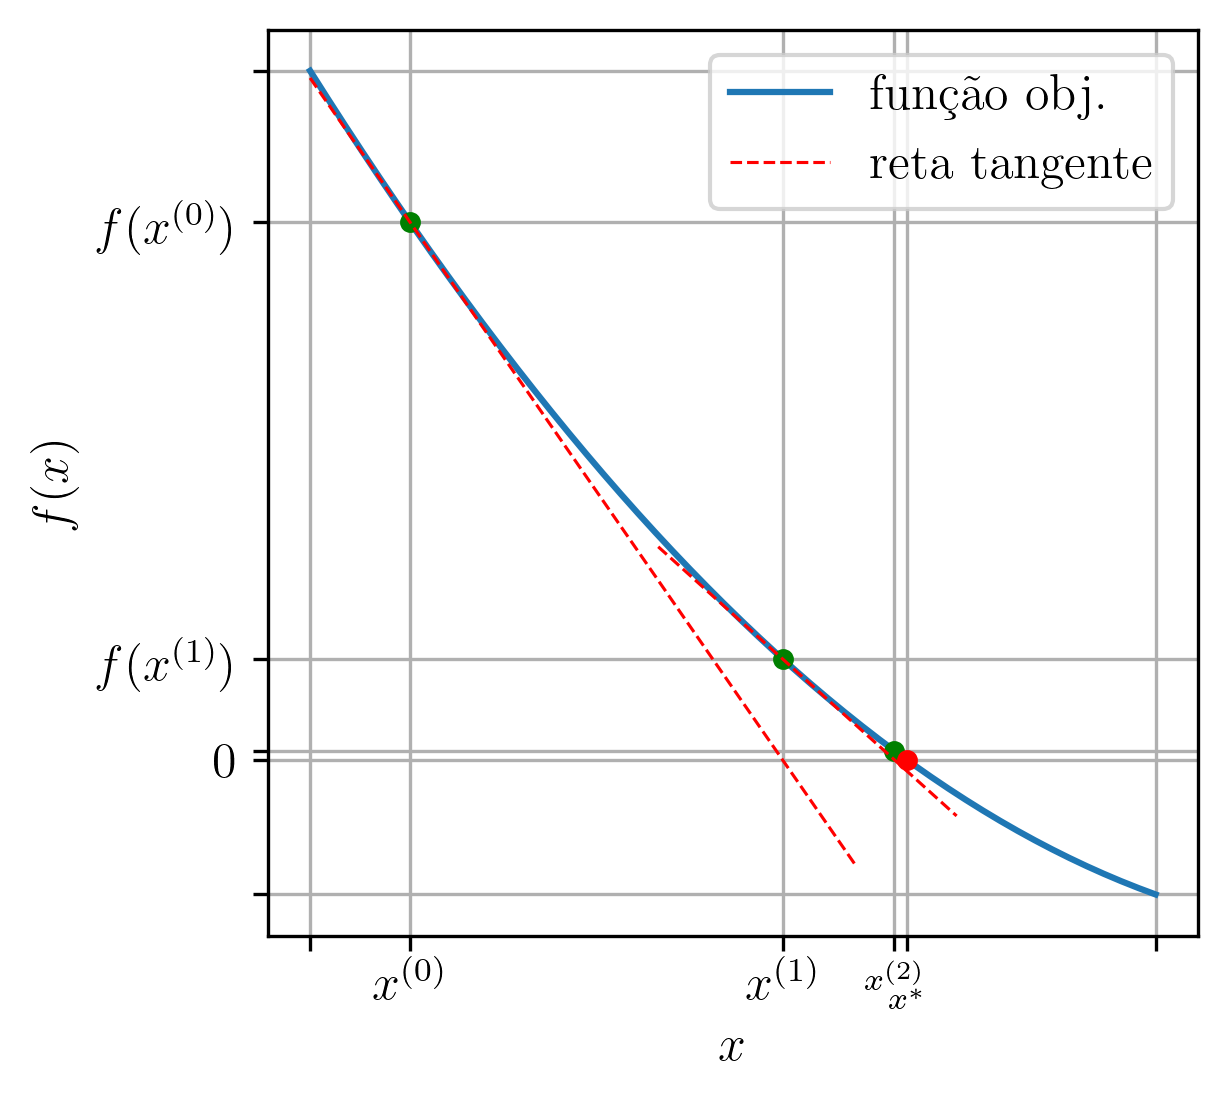
\includegraphics[width=\textwidth]{./cap_eq1d/dados/fig_Newton_geointerp/fig}
  \caption{Interpretação geométrica das iterações de Newton.}
  \label{cap_eq1d_sec_newton:fig:Newton_geointerp}
\end{figure}

Destas observações, concluímos que \hl{a iterada $x^{(k+1)}$ do método de Newton corresponde ao ponto de interseção da reta tangente ao gráfico da $f$ pelo ponto $(x^{k}, f(x^{k}))$ com o eixo das abscissas}\endnote{Eixo $x$.}. Consulte a Figura~\ref{cap_eq1d_sec_newton:fig:Newton_geointerp}.

\begin{ex}\label{cap_eq1d_sec_newton:ex:Newton_init}
  Consideremos que o método de Newton seja usado para aproximarmos o zero de
  \begin{equation}
    f(x) = (x-1)e^{-x^2}.
  \end{equation}
Observemos que esta função tem $x=1$ como seu único zero. Agora, se escolhermos $x^{(0)} = 0,5$ as iterações de Newton convergem para este zero, mas, se escolhermos $\tilde{x}^{(0)}=1,5$ não (consulte a Tabela~\ref{cap_eq1d_sec_newton:tab:ex_Newton_init}).

\begin{table}[H]
  \centering
  \caption{Resultados referentes ao Exemplo \ref{cap_eq1d_sec_newton:ex:Newton_init}}
  \label{cap_eq1d_sec_newton:tab:ex_Newton_init}
  \begin{tabular}{r|cc}
    $k$ & $x^{(k)}$   & $\tilde{x}^{(k)}$ \\\hline
    0 & $5,0000\E-1$ & $1,5000\E+0$ \\
    1 & $8,3333\E-1$ & $2,5000\E+0$ \\
    2 & $9,6377\E-1$ & $2,7308\E+0$ \\
    3 & $9,9763\E-1$ & $2,9355\E+0$ \\
    4 & $9,9999\E-1$ & $3,1223\E+0$ \\
    5 & $1,0000\E+0$ & $3,2955\E+0$ \\
  \end{tabular}
\end{table}

\begin{figure}[H]
  \centering
  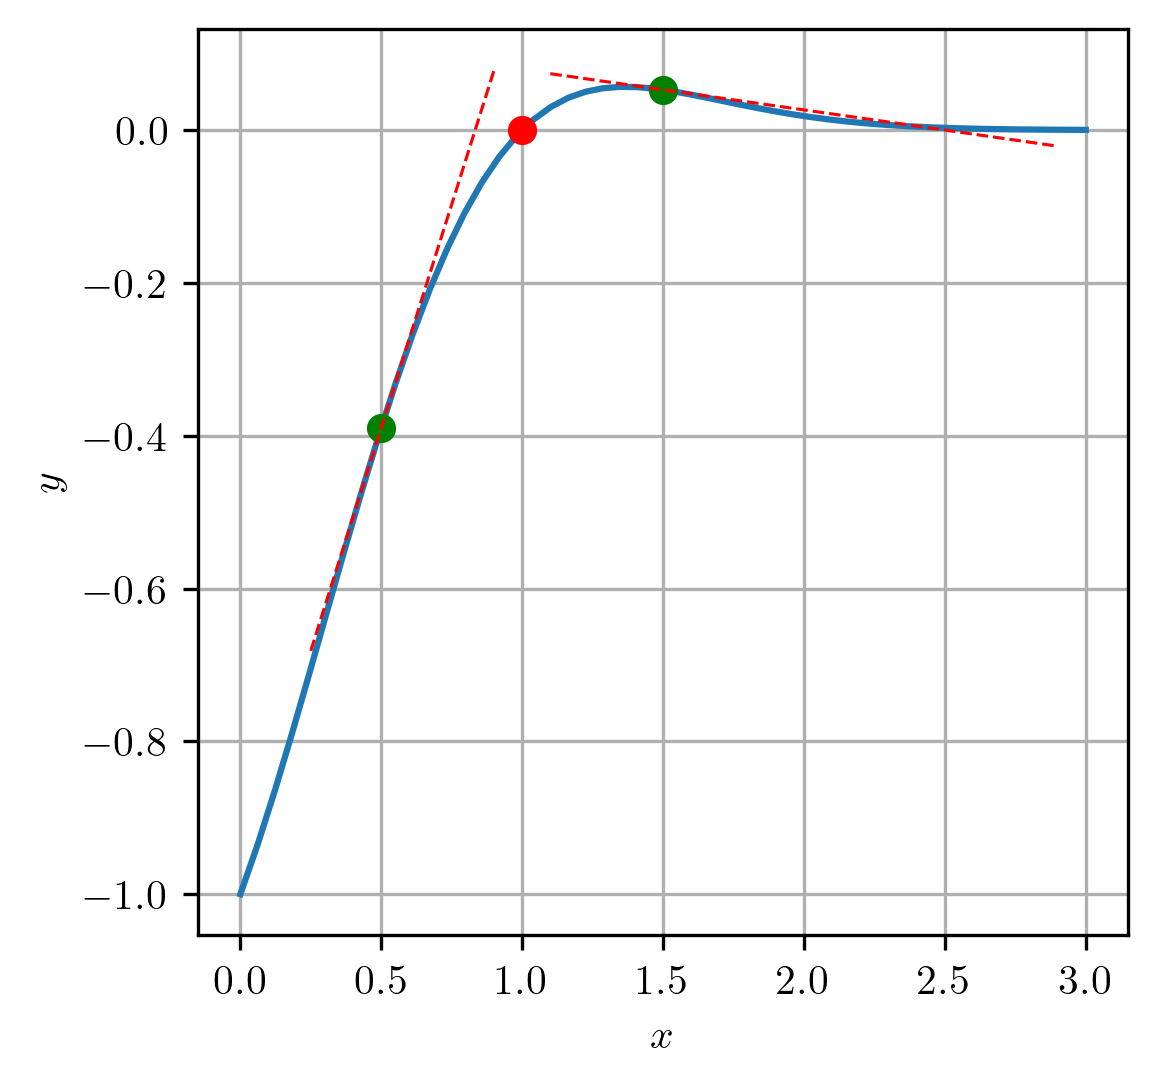
\includegraphics[width=\textwidth]{./cap_eq1d/dados/fig_newton_ex_init/fig}
  \caption{Escolha da aproximação inicial para o método de Newton.}
  \label{cap_eq1d_sec_newton:fig:ex_Newton_init}
\end{figure}

Embora ambas aproximações iniciais estão a mesma distância da solução $x=1$, quando tomamos $x^{(0)}=1,5$ as iterações irão divergir, como podemos observar da interpretação geométrica dada na Figura \ref{cap_eq1d_sec_newton:fig:ex_Newton_init}.
\end{ex}

\subsection{Análise de Convergência}

Seja $x^*$ o zero de uma dada função \hl{$f$ duas vezes continuamente diferenciável com $f'(x)\neq 0$} para todo $x\in [x^*-\varepsilon_0, x^*+\varepsilon_0]$ para algum $\varepsilon_0>0$. Seja, também, $(x^{(k)})_{k=0}^\infty$ a sequência das iteradas de Newton
\begin{equation}\label{eq:newton_iter1}
  x^{(k+1)} = x^{(k)} - \frac{f(x^{(k)})}{f'(x^{(k)})},\quad k=0, 1, 2, \ldots,
\end{equation}
com aproximação inicial $x^{(0)}\in (x^*-\varepsilon_0, x^*+\varepsilon_0)$. Então, do polinômio de Taylor de grau 1 de $f$ em torno de $x^{(0)}$, temos
\begin{equation}
  f(x^*) = f(x^{(0)}) + f'(x^{(0)})(x^* - x^{(0)}) + \frac{f''(\xi^{(0)})}{2!}(x^*-x^{(0)})^2,
\end{equation}
onde $\xi^{(0)}$ está entre $x^{(0)}$ e $\xi^{(0)}$. Daí, rearranjamos os termos e notamos que $f(x^*)=0$ para obtermos
\begin{equation}
  x^* - \left[x^{(0)} - \frac{f(x^{(0)})}{f'(x^{(0)})}\right] = \frac{f''(\xi^{(0)})}{2f'(x^{(0)})}(x^*-x^{(0)})^2.
\end{equation}
Então, da iteração de Newton \eqref{eq:newton_iter1}, temos
\begin{equation}
  x^* - x^{(1)} = \frac{f''(\xi^{(0)})}{2f'(x^{(0)})}(x^* - x^{(0)})^2
\end{equation}
Logo,
\begin{equation}\label{eq:newton_taxa_1}
  |x^* - x^{(1)}| \leq C |x^* - x^{(0)}|^2,
\end{equation}
com
\begin{equation}
  C = \sup_{x,y\in [x^*-\varepsilon, x^*+\varepsilon]} \left|\frac{f''(x)}{2f'(y)}\right|.
\end{equation}
Segue, então, que se $x^{(0)}\in (x^*-\varepsilon, x^* + \varepsilon)$ para algum $\varepsilon>0$ tal que
\begin{equation}
  C |x^* - x^{(0)}|^2 < 1,\quad\forall x\in (x^*-\varepsilon, x^* + \varepsilon),
\end{equation}
então $x^{(1)}\in (x^*-\varepsilon, x^*+\varepsilon)$.

Logo, por indução matemática\endnote{Veja o exercício \ref{ex:Newton_analise_conv}.}, temos que \hl{o método de Newton tem ordem de convergência quadrática}
\begin{equation}\label{eq:Newton_taxa_quadratica}
  \hleq{|x^{(k+1)}-x^*| \leq C|x^{(k)}-x^{*}|^{\pmb{2}}},
\end{equation}
\hl{para qualquer escolha de $x^{(0)}$ suficientemente próximo de $x^*$}, i.e. $x^{(0)}\in (x^*-\varepsilon, x^*+\varepsilon)$.

\begin{obs}
  O intervalo $(x^*-\varepsilon, x^*+\varepsilon)$ é chamado de \hl{\emph{bacia de atração} do método de Newton}.
\end{obs}

\begin{ex}\label{ex:Newton_taxa}
  Retornamos ao problema de encontrar o zero da função
  \begin{equation}
    \begin{aligned}
      f(x) &= \sen^2\left(x+\frac{\pi}{4}\right) - x^3 \\
      &+ \frac{\pi}{4}x^2 + \frac{5\pi^2}{16}x + \frac{3\pi^3}{64}.
  \end{aligned}
  \end{equation}
  no intervalo $[2,3]$. Este problema foi construído de forma que $x^* = 3\pi/4$ é um zero de $f$. Então, fazendo as iterações de Newton com aproximação inicial $x^{(0)}=2,6$, obtemos os resultados apresentados na Tabela \ref{tab:ex_Newton_taxa}, os quais evidenciam a convergência quadrática das iterações computadas.

\begin{table}[h!]
  \centering
  \caption{Resultados referentes ao Exemplo \ref{ex:Newton_taxa}.}
  \label{tab:ex_Newton_taxa}
  \begin{tabular}{r|cc}
    $k$ & $x^{(k)}$ & $|x^{(k)}-x^*|$ \\\hline
    0 & $2,6000$ & $2,4\E-01$ \\
    1 & $2,3836$ & $2,7\E-02$ \\
    2 & $2,3566$ & $3,9\E-04$ \\
    3 & $2,3562$ & $8,3\E-08$ \\
    4 & $2,3562$ & $3,6\E-15$ \\\hline
  \end{tabular}
\end{table}

\end{ex}

\subsection{Zeros Múltiplos}\index{zeros múltiplos}

Na análise de convergência acima foi necessário assumir que $f'(x) \neq 0$ para todo $x$ em uma vizinha do zero $x^*$ da função $f$. Isto não é possível no caso de $x^*$ ser um zero duplo pois, então, $f'(x^*) = 0$. Neste caso, podemos aplicar o método de Newton a $f'(x)$, a qual tem $x^*$ como um zero simples.

\begin{ex}\label{ex:Newton_multpar}
  Consideremos o problema de aproximar o zero da função
  \begin{equation}\label{cap_eq1d_sec_newton:eq:funex}
    \begin{aligned}
      f(x) &= \sen^2\left(x+\frac{\pi}{4}\right) - x^3 \\
      &+ \frac{\pi}{4}x^2 + \frac{5\pi^2}{16}x + \frac{3\pi^3}{64}.
  \end{aligned}
  \end{equation}
  no intervalo $[-1,0]$. Este problema foi construído de forma que $x^* = -\pi/4$ é um zero duplo de $f$. Então, aplicamos o método de Newton a
  \begin{equation}
    \begin{aligned}
      f'(x) &= 2\sen\left(x+\frac{\pi}{4}\right)\cos\left(x+\frac{\pi}{4}\right) \\
      &- 3x² + \frac{\pi}{2}x+\frac{5\pi^2}{16}.
  \end{aligned}
  \end{equation}
Ou seja, as iterações de Newton são
\begin{equation}
  x^{(k+1)} = x^{(k)} - \frac{f'(x^{(k)})}{f''(x^{(k)})},\quad k=0, 1, 2, \ldots,
\end{equation}
sendo $x^{(1)}$ uma aproximação inicial. Na Tabela~\ref{cap_eq1d_sec_newton:tab:ex_Newton_multpar}, temos os resultados obtidos da computação destas iterações com $x^{(1)}=-0,5$.

\begin{table}[h!]
  \centering
  \caption{Resultados referentes ao Exemplo \ref{cap_eq1d_sec_newton:ex:Newton_multpar}.}
  \label{cap_eq1d_sec_newton:tab:ex_Newton_multpar}
  \begin{tabular}{r|cc}
    $k$ & $x^{(k)}$ & $|x^{(k)}-x^*|$ \\\hline
    0 & -0.5000 & \\
    1 & -0.8341 & 3.3e-01\\
    2 & -0.7862 & 4.8e-02\\
    3 & -0.7854 & 7.9e-04\\
    4 & -0.7854 & 2.3e-07\\
    5 & -0.7854 & 1.9e-14\\\hline
  \end{tabular}
\end{table}

\end{ex}

\begin{obs}\normalfont{\hl{(Zeros múltiplos.)}}\label{cap_eq1d_sec_newton:obs:zeros_multiplos}
  No caso de zeros de multiplicidade $m>1$ de uma dada função $f$, podemos aplicar o método de Newton à derivada $m-1$ de $f$, o que requer o cálculo de $m$ derivadas de $f$. Alternativamente, consideramos aplicar o método à função auxiliar
  \begin{equation}
    \hleq\mu(x) := \frac{f(x)}{f'(x)}.
  \end{equation}
  De fato, se $x^*$ é zero de multiplicidade $m\geq 1$ de $f$, então existe uma função $g$ tal que $g(x^*)\neq 0$ e
  \begin{equation}
    f(x) = \left(x-x^*\right)^mg(x)
  \end{equation}
  Com isso, temos
  \begin{align*}
    \mu(x) &= \frac{\left(x-x^*\right)^mg(x)}{m\left(x-x^*\right)^{m-1}g(x)+\left(x-x^*\right)^mg'(x)}\\
           &= \frac{\left(x-x^*\right)g(x)}{mg(x) + \left(x-x^*\right)g'(x)}
  \end{align*}
  Como $g\left(x^*\right)\neq 0$, temos que
  \begin{equation}
    \frac{g(x^*)}{mg\left(x^*\right) + \left(x^*-x^*\right)g'\left(x^*\right)} = \frac{1}{m}\neq 0.
  \end{equation}
  Ou seja, $x^*$ é um zero simples de $\mu$. A iteração do Método de Newton aplicado à $\mu$ fornece
  \begin{align}
    x^{(k+1)} &= x^{(k)} - \frac{\mu\left(x^{(k)}\right)}{\mu'\left(x^{k+1}\right)}\\
              &= x^{(k)} = \frac{\frac{f\left(x^{(k)}\right)}{f'\left(x^{(k)}\right)}}{\frac{\left[f'\left(x^{(k)}\right)\right]^2 - f\left(x^{(k)}\right)f''\left(x^{(k)}\right)}{\left[f'\left(x^{(k)}\right)\right]^2}}
  \end{align}
  Rearranjando os termos, obtemos a \hl{iteração modificada de Newton para zeros de multiplicidade maior que 1}
  \begin{equation}\label{cap_eq1d_sec_newton:eq:iter_newton_zero_multiplo}
    \hleq x^{(k+1)} = x^{(k)} - \frac{f\left(x^{(k)}\right)f'\left(x^{(k)}\right)}{\left[f'\left(x^{(k)}\right)\right]^2 - f\left(x^{(k)}\right)f''\left(x^{(k)}\right)}.
  \end{equation}
  Para uma aplicação, consulte o exercício \ref{cap_eq1d_sec_newton:exer:iter_newton_zeros_multiplos}.
\end{obs}

\subsection*{Exercícios}

\begin{exer}\label{exer:Newton_1}
  Use o método de Newton para obter uma aproximação do zero de $f(x)=x^3\sen(x)-\cos(x)$ no intervalo $[0,5, 1]$ com precisão de $10^{-6}$.
\end{exer}
\begin{resp}
  $9,15811\times 10^{-1}$
\end{resp}

\begin{exer}\label{exer:Newton_multpar}
  Use o método de Newton para obter uma aproximação do zero de
  \begin{equation}
    \begin{aligned}
      f(x) &= (-x^2+1,154x-0,332929)\cos(x) \\
           &+ x^2 - 1,154x + 0,332929
    \end{aligned}
\end{equation}
no intervalo $(0,55, ~0,65)$ com precisão de $10^{-5}$.
\end{exer}
\begin{resp}
  $5,7700\times 10^{-1}$
\end{resp}

\begin{exer}\label{cap_eq1d_sec_newton:exer:iter_newton_zeros_multiplos}
  A função \eqref{cap_eq1d_sec_newton:eq:funex} tem um zero de multiplicidade par em $x=-\pi/4$. Assumindo a aproximação inicial $x^{(0)} = -0,5$, aplique a iteração modificada de Newton dada em \eqref{cap_eq1d_sec_newton:eq:iter_newton_zero_multiplo} e compare os resultados com apresentados na Tabela~\ref{cap_eq1d_sec_newton:tab:ex_Newton_multpar}.
\end{exer}

\begin{exer}
  Assumindo a aproximação inicial $x^{(0)} = 1$, aproxime o zero de
  \begin{equation}
    f(x) = e^x - x - 1
  \end{equation}
  usando:
  \begin{enumerate}[a)]
  \item[a)] a iteração de Newton para $f$.
  \item[b)] a iteração de Newton para $f'$.
  \item[c)] a iteração modificada de Newton\endnote{Equação~\eqref{cap_eq1d_sec_newton:eq:iter_newton_zero_multiplo}.} para $f$.
  \end{enumerate}
  Qual a melhor abordagem? Justifique sua resposta.
\end{exer}
\begin{resp}
  Dica: Analise a convergência das iteradas para cada abordagem.
\end{resp}

\begin{exer}
  Use o Método de Newton para obter a aproximação do zero de
  \begin{equation}
    p(x) = x^3 - 3\pi x^2 + 3\pi^2 x - \pi^3.
  \end{equation}
\end{exer}
\begin{resp}
  Dica: $x=\pi$ é zero de multiplicidade 3.
\end{resp}

\subsubsection{Análise Numérica}

\begin{exer}\label{ex:Newton_analise_conv}
  Complete a demonstração por indução matemática de que o método de Newton tem taxa de convergência quadrática.
\end{exer}

\ifisbook
\subsubsection{Respostas}
\shipoutAnswer
\fi

%%% SECTION %%%

\section{Método da Secante}\label{cap_eq1d_sec_secante}

\hl{O Método da Secante é um método tipo de Newton}. Observamos que para duas aproximações $x^{(k)}$ e $x^{(k-1)}$ suficientemente próximas, temos\endnote{Razão fundamental do Cálculo.}
\begin{equation}
  f'(x^{(k)}) \approx \frac{f(x^{(k)})-f(x^{(k-1)})}{x^{(k)}-x^{(k-1)}}.
\end{equation}
Assim sendo, substituindo esta aproximação na iteração de Newton (Eq. \eqref{cap_eq1d_sec_newton:eq:Newton_iteracao}), obtemos a \hl{\emph{iteração do Método da Secante}}
\begin{subequations}\label{cap_eq1d_sec_secante:eq:iter_secante}\hleq
  \begin{align}
    x^{(0)}&, x^{(1)} = \text{aprox. iniciais},\\
    x^{(k+1)} &= x^{(k)} - f(x^{(k)})\frac{x^{(k)}-x^{(k-1)}}{f(x^{(k)})-f(x^{(k-1)})},
  \end{align}
\end{subequations}
para $k=1, 2, 3, \ldots$.

\begin{ex}\label{ex:secante_exec}
  Consideramos o problema de encontrar o zero da função
  \begin{equation}
    \begin{aligned}
      f(x) &= \sen^2\left(x+\frac{\pi}{4}\right) - x^3 \\
      &+ \frac{\pi}{4}x^2 + \frac{5\pi^2}{16}x + \frac{3\pi^3}{64}.
    \end{aligned}
  \end{equation}
  no intervalo $[2,3]$. Fazendo as iterações do Método da Secante com aproximações iniciais $x^{(0)}=2,6$ e $x^{(1)}=2,5$, obtemos os resultados apresentados na Tabela \ref{cap_eq1d_sec_secante:tab:ex_secante_exec}.

\begin{table}[h!]
  \centering
  \caption{Resultados referentes ao Exemplo \ref{cap_eq1d_sec_secante:ex:secante_exec}.}
  \label{cap_eq1d_sec_secante:tab:ex_secante_exec}
  \begin{tabular}{r|ccc}
    $k$ & $x^{(k-1)}$ & $x^{(k)}$ & $|x^{(k)}-x^{(k-1)}|$ \\\hline
    0 & $2,6000$ & $2,5000$ & -x-\\
    1 & $2,5000$ & $2.3728$ & $1,3\E-1$ \\
    2 & $2,3728$ & $2,3574$ & $1,5\E-2$ \\
    3 & $2,3574$ & $2,3562$ & $1,2\E-3$ \\
    4 & $2,3562$ & $2,3562$ & $1,1\E-5$ \\
    5 & $2,3562$ & $2,3562$ & $7,0\E-9$ \\\hline
  \end{tabular}
\end{table}

\begin{lstlisting}
import numpy as np

# fun obj
f = lambda x: np.sin(x+np.pi/4)**2 \
  - x**3 + np.pi/4*x**2 + 5*np.pi**2/16*x \
  + 3*np.pi**3/64

# aprox. iniciais
x0 = 2.6
x1 = 2.5
print(f'\n0: {x0:.4f}, {x1:.4f}')

# iterações
for k in range(5):
  x = x1 - f(x1)*(x1-x0)/(f(x1)-f(x0))
  x0 = x1
  x1 = x
  print(f'{k+1}: {x0:.4f}, {x1:.4f}, {np.fabs(x1-x0):.1e}')
\end{lstlisting}

\end{ex}

\subsection{Interpretação Geométrica}

A iteração do Método da Secante é
\begin{equation}
  x^{(k+1)} = x^{(k)} - f(x^{(k)})\frac{x^{(k)}-x^{(k-1)}}{f(x^{(k)})-f(x^{(k-1)})},
\end{equation}
donde segue que
\begin{equation}
  0 = x^{(k+1)}-x^{(k)} + f(x^{(k)})\frac{x^{(k)}-x^{(k-1)}}{f(x^{(k)})-f(x^{(k-1)})},
\end{equation}
bem como que
\begin{equation}\label{cap_eq1d_sec_secante:eq:secante_geointerp}
  0 = \frac{f(x^{(k)})-f(x^{(k-1)})}{x^{(k)}-x^{(k-1)}}(x^{(k+1)}-x^{(k)}) + f(x^{(k)}).
\end{equation}
Ou seja, \hl{$x^{(k+1)}$ é o ponto de interseção} da reta
\begin{equation}
  y = \frac{f(x^{(k)})-f(x^{(k-1)})}{x-x^{(k-1)}}(x^{(k+1)}-x^{(k)}) + f(x^{(k)}).
\end{equation}
\hl{com o eixo $x$}. Esta é a \hl{reta secante ao gráfico de $f$ pelos pontos $(x^{(k)}, f(x^{(k)}))$ e $(x^{(k-1)}, f(x^{(k-1)}))$}.

\begin{figure}[H]
  \centering
  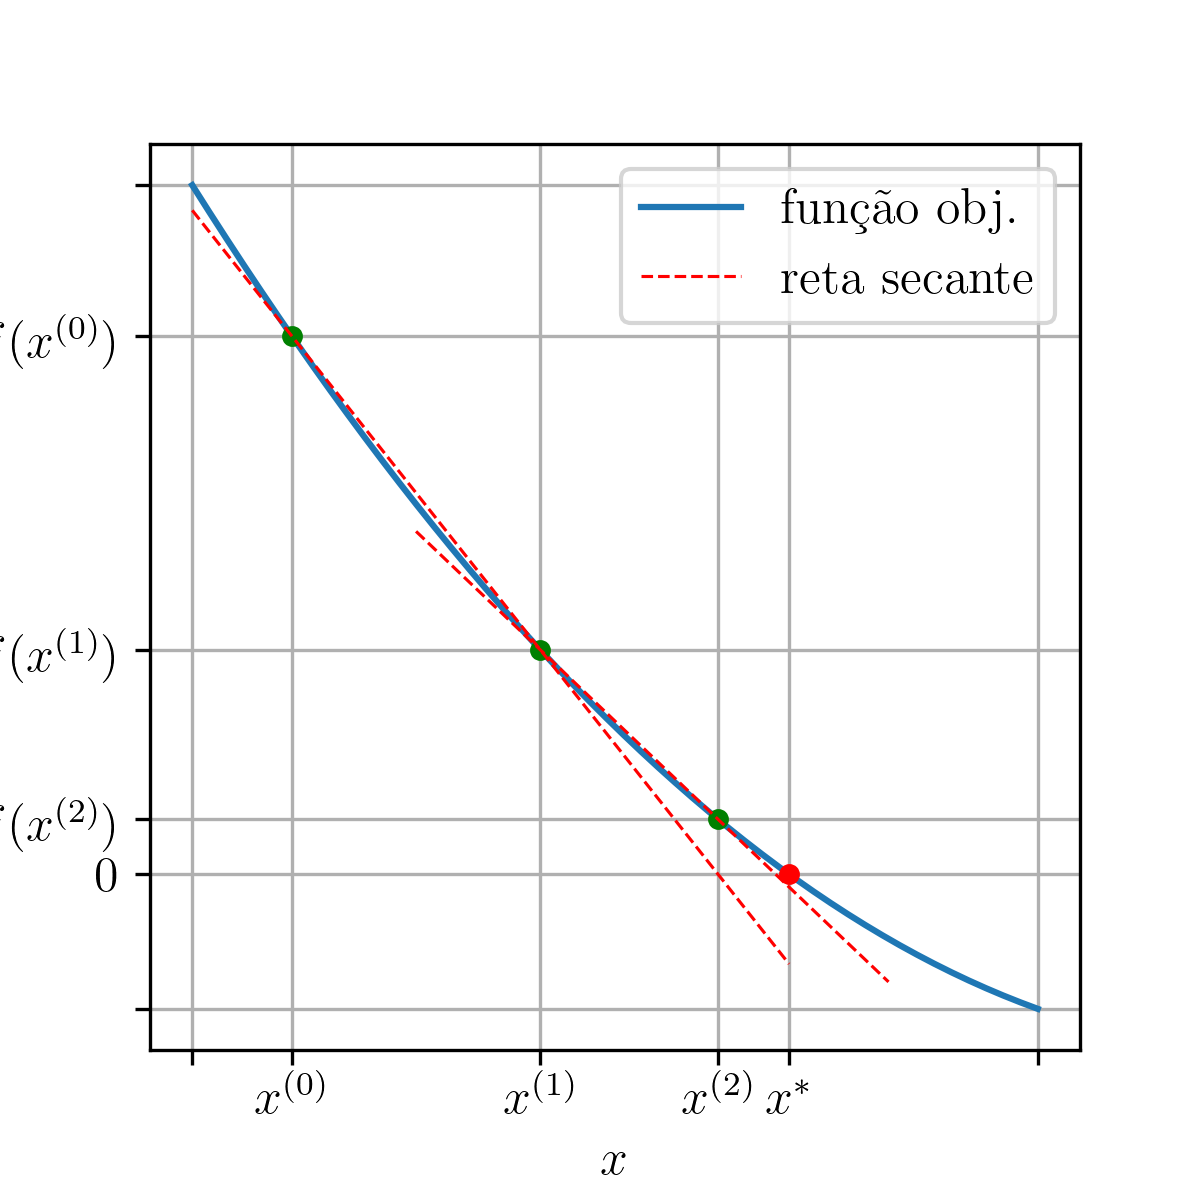
\includegraphics[width=\textwidth]{./cap_eq1d/dados/fig_secante_geointerp/fig}
  \caption{Interpretação geométrica do Método da Secante.}
  \label{cap_eq1d_sec_secante:fig:secante_geointerp}
\end{figure}


\begin{obs}\normalfont{\hl{(Aproximações iniciais.)}}
  A interpretação geométrica do método da secante pode nos ajudar a escolher as aproximações iniciais $x^{(1)}$ e $x^{(2)}$. Como uma boa prática, escolhemo-las próximas do zero (por inspeção gráfica), tomando $x^{(1)}$ como uma aproximação melhor que $x^{(0)}$. 
\end{obs}

\begin{obs}\normalfont{\hl{(Ordem de convergência super-linear.)}}
  A ordem de convergência do Método da Secante é superlinear com
  \begin{equation}\hleq
    |x^{(k+1)}-x^*| \leq C|x^{(k)}-x^*|^{\pmb{\varphi}},
  \end{equation}
  onde $\varphi = (1+\sqrt{5})/2\approx 1,618$ (\href{https://pt.wikipedia.org/wiki/Propor%C3%A7%C3%A3o_%C3%A1urea}{razão áurea}) e $x^*$ é o zero de $f$.
\end{obs}

\begin{obs}\normalfont{\hl{(Zeros de multiplicidade par.)}}
  A ordem de convergência super-linear do método da secante não se mantém para o caso de $x^*$ ser um zero múltiplo. Para contornar este problema, pode-se aplicar o método à derivada $n-1$ de $f$, a fim de se aproximar um zero de multiplicidade $n$.
\end{obs}

\begin{obs}\normalfont{\hl{(Cancelamento catastrófico.)}}
  Conforme convergem as iterações do método da secante, o denominador $f(x^{(k)})-f(x^{(k-1)})$ pode convergir rapidamente para zero, ocasionando uma divisão por zero.
\end{obs}


\subsection*{Exercícios}

\begin{exer}
  Use o Método da Secante para obter uma aproximação do zero de
  \begin{equation}
    f(x)=x^3\sen(x)-\cos(x)
  \end{equation}
  no intervalo $[0,5, 1]$ com precisão de $10^{-5}$.
\end{exer}
\begin{resp}
  $9,1581\times 10^{-1}$
\end{resp}

\begin{exer}
  Use o Método da Secante para computar a(s) solução(ões) das seguintes equações com precisão de 8 dígitos significativos.
  \begin{enumerate}[a)]
  \item $x = 2^{-x}$ para $0\leq x \leq 2$.
  \item $e^{-x^2} = 3x - x^2$ para $-1\leq x\leq 4$.
  \end{enumerate}
\end{exer}
\begin{resp}
  a) $6.4118574\times 10^{-1}$; b) $3.3536470\times 10^{-1}$; $2.9999589$
\end{resp}

\begin{exer}
  Use o Método da Secante para obter uma aproximação do zero de
  \begin{equation}
    \begin{aligned}
      f(x) &= \sen^2\left(x+\frac{\pi}{4}\right) - x^3 \\
           &+ \frac{\pi}{4}x^2 + \frac{5\pi^2}{16}x + \frac{3\pi^3}{64}.
    \end{aligned}
\end{equation}
  no intervalo $[-1, 0]$ com precisão de $10^-5$. Compare a convergência entre as seguintes abordagens:
  \begin{enumerate}[a)]
  \item aplicando a iteração \eqref{cap_eq1d_sec_secante:eq:iter_secante} diretamente à $f$.
  \item aplicando a iteração \eqref{cap_eq1d_sec_secante:eq:iter_secante} diretamente à $f'$.
  \end{enumerate}
  Qual das duas abordagens tem convergência mais rápida? Justifique sua resposta.
\end{exer}
\begin{resp}
  Dica: $f$ tem um zero de multiplicidade par no intervalo $[-1, 0]$.
\end{resp}

\begin{exer}
  Use o Sétodo da Secante para obter uma aproximação do zero de
  \begin{equation}
    \begin{aligned}
      f(x) &= (-x^2+1,154x-0,332929)\cos(x) \\
           &+ x^2 - 1,154x + 0,332929
    \end{aligned}
\end{equation}
no intervalo $[0,55, ~0,65]$ com precisão de $10^-5$.
\end{exer}
\begin{resp}
  $5,7700\times 10^{-1}$
\end{resp}

\begin{exer}
  Use o Método da Secante para encontrar uma aproximação com precisão de $4$ dígitos significativos do zero de 
  \begin{equation}
    \begin{aligned}
      f(x) &= (-x^2+1,154x-0,332929)\cos(x) + x^2 \\
      &- 1,154x + 0,332929
  \end{aligned}
  \end{equation}
  no intervalo $[-1, 0]$.
\end{exer}
\begin{resp}
  $-7,861\times 10^{-1}$
\end{resp}
bootstra
\begin{exer}
  Use o Método da Secante para encontrar o ponto crítico\endnote{Definimos que $x$ é ponto crítico de uma dada $f$, quando $f'(x) = 0$ ou $\nexists f'(x)$.} de
  \begin{equation}
    f(x) = (1-x^2)e^{-x^2}
  \end{equation}
  no intervalo $[0, 2]$. Obtenha o resultado com precisão de $5$ dígitos significativos por arredondamento.
\end{exer}

\ifisbook
\subsubsection{Respostas}
\shipoutAnswer
\fi

%%% SECTION %%%

\section{Raízes de Polinômios}\label{cap_eq1d_sec_raizes}\index{raízes de!polinômios}
\badgeRevisar

Nesta seção, veremos como o método de Newton pode ser aplicado de forma robusta a polinômios com o auxílio do método de Horner\endnote{William George Horner, matemático britânico, 1786 - 1837. Fonte: \href{https://en.wikipedia.org/wiki/William_George_Horner}{Wikipedia}}. A questão central é que dado um polinômio de grau $n$ escrito na forma
\begin{equation}
  p(x) = a_{1}x^n + a_{2}x^{n-1} + \cdots + a_nx + a_{n+1},
\end{equation}
o procedimento de avaliá-lo em um ponto requer $n!n$ multiplicações e $n$ adições. Desta forma, a aplicação do método de Newton para obter as raízes de $p$ torna-se computacionalmente custosa, por requer a avaliação de $p$ e de sua derivada a cada iteração. Agora, o método de Horner nos permite avaliar $p$ em um ponto qualquer usando apenas $n$ multiplicações e $n$ adições, reduzindo enormemente o custo computacional.

\subsection{Método de Horner}\index{método de!Horner}
\badgeRevisar

Sejam dados um número $x_0$ e um polinômio de grau $n$
\begin{equation}\label{eq:Horner_poli}
  p(x) = p_1x^n + p_2x^{n-1} + \cdots + p_{n}x + p_{n+1}s.
\end{equation}
O método de Horner consiste em computar $p(x_0)$ pela iteração
\begin{align}
  q_1 &= p_1,\label{eq:Horner_b1}\\
  q_{k} &= p_k + q_{k-1}x_0,\quad k=2,3,\dotsc,n+1,\label{eq:Horner_b2}
\end{align}
sendo que, então, $p(x_0) = q_{n+1}$ e, além disso,
\begin{equation}\label{eq:Horner_decomp}
  p(x) = (x-x_0)q(x) + q_{n+1},
\end{equation}
com
\begin{equation}
  q(x) = q_1x^{n-1} + q_2x^{n-2} + \cdots + q_{n-1}x + q_{n}.
\end{equation}

De fato, a verificação de \eqref{eq:Horner_decomp} é direta, uma vez que
\begin{align}
  (x-x_0)q(x)+q_{n+1} &= (x-x_0)(q_1x^{n-1} + q_2x^{n-2} + \cdots + q_{n-1}x + q_{n})\nonumber\\ 
                      &+ q_{n+1}\\
                      &= q_1x^n + (q_2-q_1x_0)^{n-1} + \cdots + (q_{n+1}-q_{n}x_0).
\end{align}
E, então, igualando a $p(x)$ na forma \eqref{eq:Horner_poli}, temos as equações \eqref{eq:Horner_b1}-\eqref{eq:Horner_b2}.

\begin{ex}\label{ex:Horner_exec}
  Consideremos o polinômio
  \begin{equation}
    p(x) = x^3 - 3x^2 + 4.
  \end{equation}
  Para computarmos $p(1)$ pelo método de Horner, tomamos $x_0=1$, $q_1=p_1=1$ e
  \begin{align}
    q_2 &= p_2 + q_1x_0 = -3 + 1\cdot 1 = -2\\
    q_3 &= p_3 + q_2x_0 = 0 + (-2)\cdot 1 = -2\\
    q_4 &= p_4 + q_3x_0 = 4 + (-2)\cdot 1 = 2.
  \end{align}
Com isso, temos $p(3) = q_4 = 4$ (verifique!).

% \ifisoctave
% Para este caso, podemos implementar o método de Horner no \verb+GNU Octave+ com o seguinte \href{https://github.com/phkonzen/notas/blob/master/src/MatematicaNumerica/cap_eq1d/dados/ex_Horner_exec/ex_Horner_exec.m}{código}:
% \verbatiminput{./cap_eq1d/dados/ex_Horner_exec/ex_Horner_exec.m}
% \fi
\end{ex}

\begin{obs}\label{obs:Horner_polider}
  Ao computarmos $p(x_0)$ pelo método de Horner, obtemos a decomposição
  \begin{equation}
    p(x) = (x-x_0)q(x) + b_{n+1}.
  \end{equation}
Desta forma, temos
\begin{equation}
  p'(x) = q(x) + (x-x_0)q'(x),
\end{equation}
donde temos que $p'(x_0) = q(x_0)$. Com isso, para computarmos $p'(x_0)$ podemos aplicar o método de Horner a $q(x)$.

% \ifisoctave
% A implementação do método de Horner no \verb+GNU Octave+ para computar $p(x_0)$ e $p'(x_0)$ pode ser feita com o seguinte \href{https://github.com/phkonzen/notas/blob/master/src/MatematicaNumerica/cap_eq1d/dados/obs_Horner_fun/Horner.m}{código}:
% \verbatiminput{./cap_eq1d/dados/obs_Horner_fun/Horner.m}
% \fi
\end{obs}

\subsection{Método de Newton-Horner}
\badgeRevisar

A implementação do método de Newton a polinômios pode ser feita de forma robusta com o auxílio do método de Horner. Dado um polinômio $p$ e uma aproximação inicial $x^{(1)}$ para uma de suas raízes reais, a iteração de Newton consiste em
\begin{equation}
  x^{(k+1)} = x^{(k)} - \frac{p(x^{(k)})}{p'(x^{(k)})},
\end{equation}
na qual podemos utilizar o método de Horner para computar $p(x^{(k)})$ e $p'(x^{(k)})$.

\begin{ex}\label{ex:poli_Newton}
  Consideremos o caso de aplicar o método de Newton para obter uma aproximação da raiz $x=-1$ de
  \begin{equation}
    p(x) = x^3 - 3x^2 + 4,
  \end{equation}
  com aproximação inicial $x^{(1)} = -2$. Na Tabela \ref{tab:ex_poli_Newton} temos os resultados obtidos.

\begin{table}[h!]
  \centering
  \caption{Resultados referentes ao Exemplo \ref{ex:poli_Newton}.}
  \label{tab:ex_poli_Newton}
  \begin{tabular}{r|cc}
    $k$ & $x^{(k)}$ & $|x^{(k)}-x^{(k-1)}|$ \\\hline
    1 & $-2,0000$ & -x- \\
    2 & $-1,3333$ & $6,7\E-1$ \\
    3 & $-1,0556$ & $2,8\E-1$ \\
    4 & $-1,0019$ & $5,4\E-2$ \\
    5 & $-1,0000$ & $1,9\E-3$ \\\hline
  \end{tabular}
\end{table}

\end{ex}

\subsection{Exercícios}

\badgeRevisar

\begin{exer}
  Use o método de Newton-Horner para computar a aproximação da raiz de $p(x) = x^3 - 3x^2 + 4$ no intervalo $[1,3]$. Observe que $p$ tem um zero duplo deste intervalo.
\end{exer}
\begin{resp}
  % \ifisoctave 
  % \href{https://github.com/phkonzen/notas/blob/master/src/MatematicaNumerica/cap_eq1d/dados/exer_NewtonHorner_multpar/exer_NewtonHorner_multpar.m}{Código.} 
  % \fi
  $2$
\end{resp}

\ifisbook
\subsubsection{Respostas}
\shipoutAnswer
\fi

%%% SECTION %%%